% \documentclass[12pt,dvipdfmx]{report}
\documentclass[12pt,dvipdfmx,twoside,openright]{report}

\usepackage[utf8]{inputenc}
\usepackage{amsmath}
\usepackage{amssymb}
\usepackage{algorithm2e}
\usepackage{algpseudocode}
\usepackage[dvipdfmx]{graphicx}
\usepackage{bm}
\usepackage{braket}
\usepackage{graphicx}
% \usepackage[margin=3cm]{geometry}
\usepackage{multicol}
\usepackage{mathtools}
\usepackage{listings,jvlisting} 
\usepackage{here}
\usepackage{longtable}
\usepackage{url}
\usepackage{comment}
\usepackage{booktabs}
\usepackage{pdfpages}
\usepackage{tikz}

\usepackage{hyperref}  % ハイパーリンクを有効化
\hypersetup{
    colorlinks=true,    % リンクをカラーで表示
    linkcolor=blue,     % 目次や章見出しのリンクの色
    urlcolor=blue,      % URLのリンク色
    citecolor=blue      % 引用のリンク色
}


\renewcommand{\maketitle}{
    \begin{center}
        \vspace*{2cm}
        {\LARGE \textbf{A MASTER THESIS}} \\[2cm]  % 修士論文
        {\Huge \textbf{Embedding of Tree Tensor Networks into Quantum Circuits of Two-Qubit
Gates}} \\[0.5cm]  % 英語タイトル
        {\Large 二量子ビットゲート量子回路へのツリーテンソルネットワークの埋め込み} \\[2cm]  % 日本語タイトル
        {\small January 2025} \\[1cm]  % 日時
        {\large Supervisor: Prof. Synge Todo} \\[2cm]  % 指導教員名
        \rule[0.5ex]{10cm}{1pt} \\  % 上の線
        {\large Shota Sugawara} \\ % 名前
        \rule[0.5ex]{10cm}{1pt} \\[1cm]  % 下の線
        {\large Department of Physics, Graduate School of Science \\ The University of Tokyo}  % 所属
    \end{center}
    \thispagestyle{empty} 
}


% \title{Embedding of Tree Tensor Networks into Shallow Quantum Circuits}


% \author{Shota Sugawara}
% \date{2025/1/6}

\begin{document}

\maketitle

% \clearpage
% \thispagestyle{empty}
% \mbox{}
% \newpage

\cleardoublepage
\chapter*{Acknowledgments}
\thispagestyle{empty} 
This work is fully supervised and supported by Professor Synge Todo.
He dedicated a significant amount of time to my research, from discussing physics to debugging code.
Without his support, I would not have been able to complete my master's thesis.
Additionally, he taught me many important life lessons, such as how to manage projects, handle failures, and think when faced with difficulties.
What I learned from him will be a valuable guide for my future life.
Thanks to him, the two years of my master's program became an invaluable and precious time.

I am profoundly thankful to Project Associate Professor Tsuyoshi Okubo.
He also dedicated a significant amount of time to my research and made substantial contributions. 
Not only during the regular meetings but whenever I had questions, he would always use his deep knowledge of physics to accurately resolve my questions. 
It is thanks to him that I have gained a solid understanding of tensor networks.

I would also like to thank the other members of the Todo Group. 
Kazuki Inomata was responsible for part of the implementation of the research and made a significant contribution to its progress. 
Keisuke Murota and Takumi Kobori engaged in deep discussions about the relationship between tensor networks and quantum circuits. 
Tokinori Oe, as a fellow lab member, always helped me through difficult times. Additionally, I had regular discussions with Hidemaro Suwa, Masahiko Yamada, Sayan Mukherjee, Atsushi Iwaki, Tatsuya Sakashita, Keiichi Tamai, Tohru Mashiko, Yuma Nakanishi, Rihito Sakurai, Shinichiro Akiyama, Xun Zhao, Hopai Kwok, Sora Shiratani, Soichiro Imamura, Ruixiao Cao, Kazushige Ueda, and Ruqing Xu during our meetings. Their broad knowledge of physics was very stimulating for me. 
Emi Shimoshikiryo supported research activities and helped me as the secretary of the Todo Group. 
Their help always helped me a lot.

Finally, I would like to express my most profound appreciation to my family.
Thanks to my father, Mitsuru Sugawara, my mother, Yuka Sugawara, and my sister, Yumeka Sugawara, our home is always filled with laughter, allowing me to conduct my research in a mentally stable state. 
I was able to complete my master's thesis successfully because of them. 
I also want to express my deep gratitude to my grandmother, Miyoko Iwasaki, who passed away during my university years. 
She always supported me and celebrated my successes as if they were her own. 
The love she gave me continues to be a source of strength for me.

\bigskip
\begin{flushright}
\textit{Shota Sugawara}
\end{flushright}
\thispagestyle{empty} 

\cleardoublepage
\begin{abstract}
    Variational Quantum Algorithms (VQAs) are highlighted as key algorithms for demonstrating a quantum advantage on Noisy Intermediate-Scale Quantum (NISQ) devices, which are limited to executing shallow quantum circuits because of noise.
However, the barren plateau problem, where the amplitude of the loss function gradient becomes exponentially small with system size, hinders this goal.
Recent studies suggest that embedding tensor networks into quantum circuits and initializing the parameters can avoid the barren plateau.
Yet, embedding tensor networks into quantum circuits is generally difficult, and methods have been limited to the simplest structure, Matrix Product States~(MPSs).
This study proposes a method to embed Tree Tensor Networks~(TTNs), characterized by their hierarchical structure, into shallow quantum circuits.
TTNs are suitable for representing two-dimensional systems and systems with long-range correlations, which MPSs are inadequate for representing.
Our numerical results show that embedding TTNs provides better initial quantum circuits than MPS.
Additionally, our method has a practical computational complexity, making it applicable to a wide range of TTNs.
This study is expected to extend the application of VQAs to two-dimensional systems and those with long-range correlations, which have been challenging to utilize.
\end{abstract}

% \clearpage
% \thispagestyle{empty}
% \mbox{}
% \newpage

\tableofcontents
\thispagestyle{empty}


% \clearpage
% \thispagestyle{empty}
% \mbox{}
% \newpage



\cleardoublepage
\chapter{Introduction}
Variational Quantum Algorithms~(VQAs) are the foremost approach for achieving a quantum advantage with the current generation of quantum computing technologies.
Quantum computers are anticipated to outperform classical ones, with some algorithms already proving more efficient~\cite{shor1994algorithms,grover1996fast}.
However, the currently available Noisy Intermediate-Scale Quantum~(NISQ) devices cannot execute most algorithms due to their limited number of qubits and susceptibility to noise~\cite{nisq}.

VQAs are hybrid methods in which classical computers optimize parameters of quantum circuits' ansatz to minimize the cost function evaluated by quantum computers.
VQAs require only shallow circuits, making them notable as algorithms that can be executed on NISQ devices.
VQAs come in many forms, such as Quantum Machine Learning~(QML)~\cite{qml0,qml1,qml2}, Variational Quantum Eigensolver~(VQE)~\cite{vqe0,vqe1,vqe2}, and Quantum Approximate Optimization Algorithm~(QAOA)~\cite{qaoa0,qaoa1,qaoa2}, with potential applications across diverse industries and fields.

However, a significant challenge known as the barren plateau stands in the way of realizing quantum advantage~\cite{barrenplateau1,barrenplateau2}.
The barren plateau phenomenon refers to the difficulty in VQAs where the amplitude of the cost function gradient decreases exponentially as the system size increases.
This phenomenon occurs regardless of whether the optimization method is gradient-based~\cite{gradient-based} or gradient-free~\cite{gradient-free}, and it has been observed even in shallow quantum circuits~\cite{barrenplateau-shallow}.
Furthermore, it has been confirmed that this phenomenon also occurs in practical tasks using real-world data~\cite{barren-generic0,barren-generic1,barren-generic2}.
Avoiding the barren plateau is a critical challenge in demonstrating the superiority of quantum algorithms using NISQ devices.
To avoid the barren plateau, appropriate parameter initialization in VQAs is crucial since randomly initializing the parameters can result in the algorithm starting far from the solution or near a local minimum~\cite{qaoa2}.
Although various initialization methods have been considered~\cite{avoid-barren0,avoid-barren1,avoid-barren2}, using tensor networks is natural due to their compatibility with quantum circuits.

Tensor networks are originally developed to represent quantum many-body wave functions efficiently.
Any quantum circuit can be naturally regarded as a tensor network~\cite{tn-qc}, and it is sometimes possible to simulate quantum computers with a practical amount of time using tensor networks~\cite{google-ibm}.
Moreover, their utility has been recognized and applied in recent years across various fields, such as machine learning~\cite{tnml} and language models~\cite{tnlanguage}.

In this study, we focus particularly on Matrix Product States~(MPSs) and Tree Tensor Networks~(TTNs), two of the various structures of tensor networks.
MPSs are one-dimensional arrays of tensors.
Its simplest and easiest-to-use structure, along with the presence of advanced algorithms such as Density Matrix Renormalization Group~(DMRG)~\cite{dmrg}, and Time-Evolving Block Decimation~(TEBD)~\cite{tebd}, has led to its application across a wide range of fields.
These excellent algorithms have recently been applied to machine learning, continuing the exploration of new possibilities~\cite{MPSsupervised,MPSgenerative}.
On the other hand, TTNs have tree-like structures of tensors.
The procedures used in DMRG and TEBD have been applied to TTNs~\cite{dmrg-ttn,tebd-ttn}.
Additionally, the distance between any pair of leaf nodes scales in logarithmic order in TTNs, while it scales in linear order in MPSs.
As connected correlation functions decay exponentially with path length within a tensor network generally, TTNs are better suited to capture longer-range correlations and represent two-dimensional objects than MPSs.
TTNs are utilized in various fields such as chemical problems~\cite{chemical1,chemical2}, condensed matter physics~\cite{condmat1,condmat2,condmat3}, and machine learning~\cite{ml1,ml2}.

\cite{rudolph2023synergistic} has successfully avoided the barren plateau problem by utilizing tensor networks.
They proposed a method of first optimizing tensor networks, then mapping the optimized tensor networks to quantum circuits, and finally executing VQAs.
While numerical results have shown that this method can indeed avoid the barren plateau, mapping tensor network states into shallow quantum circuits is a general challenge.
The case where the tensor network structure is an MPS has already been well-studied~\cite{EncodingMPS,mpsdecomp,mpsoptim,mpspreparation}.
However, effective methods for mapping tensor networks other than MPSs to shallow quantum circuits have not yet been devised.
\begin{figure}
    \centering
    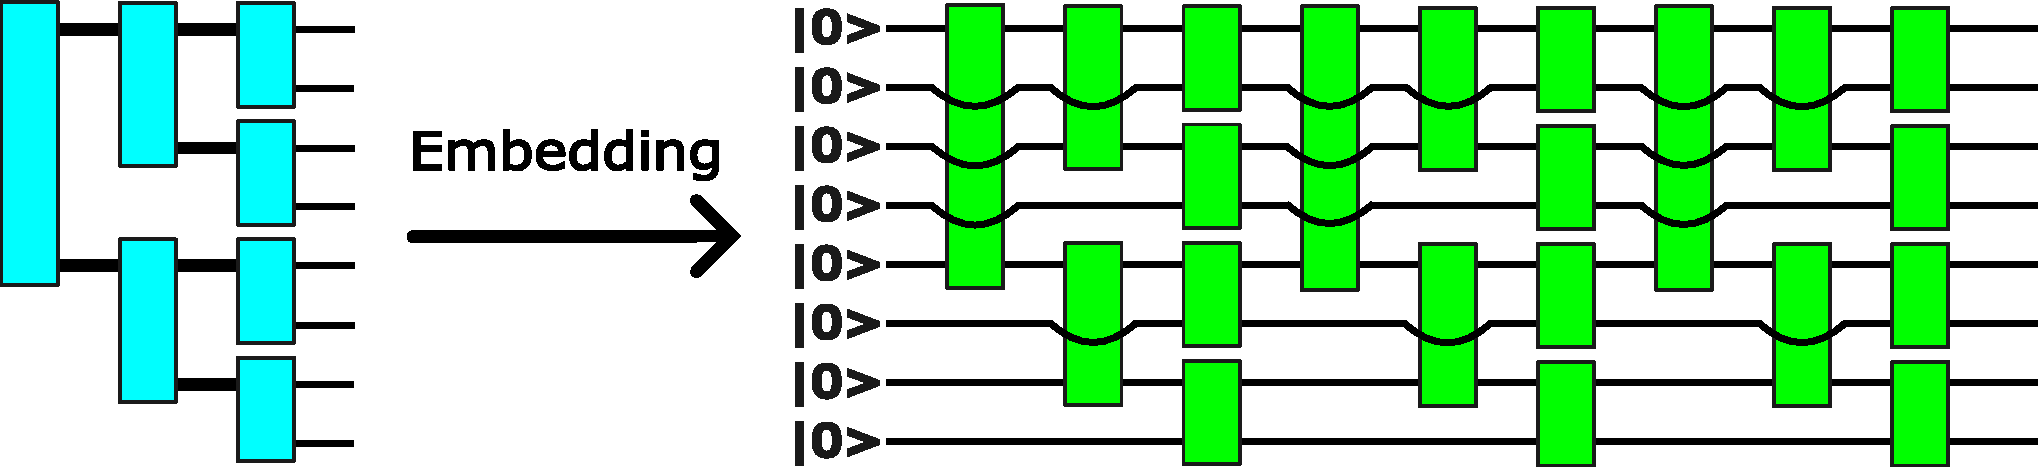
\includegraphics[width=\linewidth]{fig-task-setting.pdf}
    \caption{A schematic diagram illustrating the embedding of a TTN into a shallow quantum circuit composed solely of two-qubit gates. The aim is to ensure that the quantum state output by the quantum circuit closely approximates the quantum state represented by the TTN. The diagram depicts a case with three layers, and the approximation accuracy improves as the number of quantum circuit layers increases.}
    \label{fig:task-setting}
\end{figure}

In this thesis, we propose a method to embed TTNs into shallow quantum circuits composed of only two-qubit gates, as shown in Fig.~\ref{fig:task-setting}.
The primary obstacle to embedding TTNs into shallow quantum circuits has been the complexity of contractions arising from the intricate structure of TTNs.
In general, the contraction of tensor networks requires an exponentially large memory footprint relative to the number of qubits if performed naively.
Furthermore, determining the optimal contraction order for tensor networks is an NP-complete problem~\cite{np-complete}.
Through the innovative design of a contraction method that balances minimal approximation error and computational efficiency, we successfully extend the embedding method of MPSs~\cite{mpsdecomp} to TTNs.
Additionally, by applying the proposed method to practical problems, we successfully prepare better initial quantum circuits for VQAs than those provided by MPSs with a practical computational complexity.
This study is expected to extend the application of VQAs to two-dimensional systems and those with long-range correlations, which have previously been challenging to utilize.

\cleardoublepage
\chapter{Variational quantum algorithms}
\section{Advantages of quantum computers}
% 量子コンピュータの概要
% 量子コンピュータと古典コンピュータの違い
Quantum computers operate based on principles entirely different from classical computers, which are currently widespread globally.
Although there are numerous challenges to be addressed in both software and hardware before quantum computers can be as ubiquitously used as classical computers, their immense potential has garnered significant global interest. 
It remains uncertain whether quantum computers will eventually solve problems that classical computers cannot, but many scientists are actively conducting extensive research on the subject.

% 量子優位性を期待できる理由1: 量子コンピュータを古典でシミュレートすることの大変さ
There are two reasons to believe that quantum computers can perform tasks beyond classical computers' capabilities.
The first is that classical algorithms capable of simulating quantum computers are still unknown.
Generally, to accurately represent the quantum state of $n$ qubits on a classical computer, it is necessary to maintain $2^n$ elements.
Storing all the elements becomes fundamentally impossible as the number of qubits increases.
For example, describing a quantum state with a few hundred qubits may require more bits than the number of atoms in the universe.
Despite decades of effort by physicists and computer scientists, we still cannot simulate large-scale quantum computers using classical computers.

% 量子優位性を期待できる理由2: 計算量理論の観点
% 量子優位性を期待できる理由3: 実際に古典より良い計算量で解くアルゴリズムが考案されていること
The second is that we know specific problems that are difficult to solve with classical computers but can be efficiently addressed by quantum computers.
The most renowned example is Shor's algorithm~\cite{shor1994algorithms}, which can factorize huge composite numbers with remarkable speed.
Factoring such large numbers is challenging for classical computers and is used in cryptography due to this difficulty.
However, it has been theoretically demonstrated that quantum computers can solve this problem in polynomial time.
Although current quantum computers have only achieved the factorization of small numbers, it is anticipated that as the number of usable qubits increases, they will be able to factorize the large numbers used in cryptography.
This advancement is expected to have a significant societal impact.

Another well-known algorithm is Grover's algorithm~\cite{grover1996fast}, which enables rapid search of specific data within unsorted databases.
When using classical computers, finding a target data point in an unsorted database requires $\mathcal{O}(N)$ queries, where $N$ is the number of data points.
In contrast, Grover's algorithm can locate the target with $\mathcal{O}(\sqrt{N})$ queries, achieving quadratic speedup.
By leveraging Grover's algorithm, the exhaustive search components of various classical algorithms can be accelerated, making it applicable to problems such as satisfiability and searching for original values from specific hash values.
The latter application has even been proposed for speeding up Bitcoin mining~\cite{bitcoin}.



% 量子コンピュータの応用に関する期待

\section{Limitations of NISQ devices}
% qubitは外部のノイズの影響を受けやすいこと
While there are high expectations for the realization of quantum computers, achieving practical quantum computers will take a long time.
The core of the problem stems from the fundamental requirements inherent in the realization of quantum computers.
The first requirement is the isolation requirement.
Quantum systems must be nearly perfectly isolated to store and process information reliably.
The second requirement is the interaction requirement.
Qubits need to interact with each other strongly to process information.
With current quantum technologies, building a quantum system that meets both requirements is very challenging.

% 実用的な量子コンピュータ実現のためには誤り訂正を載せることが不可欠であること
Eventually, we expect that quantum error correction will allow us to protect and scale up quantum computers.
The principle of quantum error correction involves encoding quantum information in a highly entangled state, which prevents the environment from accessing and damaging the encoded information, thereby protecting the quantum system.
Quantum error correction techniques have been extensively studied, and many promising methods exist.
However, quantum error correction entails significant overhead, meaning that to protect quantum information, we need to use many more physical qubits than the logical qubits we want to safeguard.
This extra requirement of physical qubits increases the complexity and resources needed, making it challenging to build reliable quantum computers.

% NISQデバイスの概要(nisq4.1)
% NISQデバイスの特徴1: qubit数が少ないこと
% NISQデバイスの特徴2: ノイズが大きいこと
NISQ devices refer to Noisy Intermediate-Scale Quantum devices, widely recognized as the current state of quantum computing technology.
NISQ devices have two limitations compared to the ideal quantum computers.
First, they have a limited number of qubits, typically in several hundreds.
Consequently, they cannot execute general quantum algorithms that require many qubits.
However, this number is still promising as it exceeds what can be simulated by brute force using the most powerful existing digital supercomputers.
Second, NISQ devices are characterized by significant noise and high error rates.
As a result, it is generally expected that these noisy devices cannot execute deep circuits, such as the circuit with one thousand fundamental two-qubit operations, since the noise will overwhelm the signal.
Although NISQ devices are still in the developmental stages of quantum technology, they are garnering attention as a crucial step towards the more powerful quantum technologies that will be developed.

% NISQデバイスでは誤り訂正を載せられないこと
% NISQデバイスでは実行可能なアルゴリズムが限られること
Given the high error rates and significant noise in NISQ devices, it might seem essential to incorporate quantum error correction. 
However, error correction cannot be implemented due to the limited number of qubits in NISQ devices.
Consequently, most quantum algorithms cannot be executed on NISQ devices. 
For instance, practical applications of Grover's algorithm~\cite{grover1996fast} or Shor's algorithm~\cite{shor1994algorithms} are unlikely to be feasible. 
Nevertheless, there is considerable interest in quantum-classical hybrid algorithms, which collaborate with classical devices for computation. 
VQAs are a prominent example of such algorithms that can operate on NISQ devices.

\section{Overview of VQAs}
% vqaは広範に使える手法であること(vqa6250)
VQAs are the top proposal for achieving quantum advantage with NISQ devices. 
VQAs are similar to successful machine-learning methods like neural networks.
Furthermore, VQAs utilize classical optimization techniques by employing parameterized quantum circuits on the quantum computer and outsourcing the parameter optimization to a classical computer.
Unlike quantum algorithms for the fault-tolerant era, this keeps the quantum circuit depth shallow, reducing noise.

% vqaの手法の概要(vqa6260)
One of the primary advantages of VQAs is their ability to provide a general framework applicable to a wide range of problems.
Despite their different algorithmic structures and complexities, most VQAs share basic elements.
The initial step is to define a cost function $C(\cdot )$ that encodes the problem's solution. 
Subsequently, an ansatz is proposed, a quantum operation dependent on a set of continuous or discrete parameters $\theta$ that can be optimized. 
This ansatz is then trained in a hybrid quantum-classical loop to solve the optimization task by minimizing the cost function,
\begin{equation}
    \theta^* = \arg \min_\theta C(\theta).
\end{equation}
VQAs are unique in using quantum computers to estimate the cost function $C(\theta)$ while leveraging classical optimizers to train the parameters $\theta$.

% cost functionについてより詳しく
A key part of a VQA is encoding the problem into a cost function. 
Like classical machine learning, the cost function maps the trainable parameters $\theta$ to real numbers. 
More abstractly, it creates a hypersurface, usually called the cost landscape, where the optimizer's job is to navigate this landscape to find the global minimum.
The cost function is generally expressed as
\begin{equation}
    C(\theta ) = f(\{\rho_k\},\{O_k\},U(\theta)),
\end{equation}
where f is a function, $U(\theta)$ is a parameterized unitary, $\theta$ includes discrete and continuous parameters, $\{\rho_k\}$ are input states from a training set, and $\{O_k\}$ are a set of observables.

The cost function for VQAs should meet several key criteria: it must be faithful, efficiently estimable, provide quantum advantages, be operationally meaningful, and trainable.
Specifically, the minimum of $C(\theta )$ should correspond to the problem's solution, ensuring it is faithful.
It should be measurable on a quantum computer with possible classical post-processing, making it efficiently estimable. 
Additionally, it should not be efficiently computable with a classical computer to ensure quantum advantage. 
Smaller cost values should indicate better solution quality, making it operationally meaningful. 
Finally, it should be possible to optimize the parameters $\theta$ efficiently, ensuring the cost function is trainable.
Designing a cost function that optimally satisfies these requirements is crucial in VQA.

% ansatzについて
Another key aspect of VQA is its ansatz. 
Generally, the ansatz's form determines the parameters $\theta$ and their training process to minimize costs. 
The specific structure of an ansatz typically depends on the task, as problem-specific information can often be used to customize the ansatz. 
These are referred to as problem-inspired ansatzes.
Conversely, some ansatz architectures are problem-agnostic, meaning they can be applied even without relevant information.

Here, we review several significant ansatzes. 
The first is the hardware-efficient ansatz. 
The hardware-efficient ansatz is designed to reduce the circuit depth needed for implementation on specific quantum hardware.
The second is the variable structure ansatz. 
The variable structure ansatz optimizes not only the parameters of the circuit but also the structure of the circuit itself during training.
The third is the hybrid ansatzes. 
The hybrid ansatzes delegate part of the ansatz to classical hardware, reducing the complexity of quantum computations. By incorporating classical hardware, the computational burden on quantum systems is alleviated. 
Finally, the fourth is the TN-inspired ansatz.
The tensor network-inspired ansatz draws inspiration from tensor network theory, leveraging its extensive experience to enhance expressiveness and achieve efficient representations.

% optimizerについて

\section{Examples of VQAs}
% VQAにはたくさんの応用があることを引用して示す(vqaのApplicationsの節)
The main benefit of the VQA paradigm is its support for task-oriented programming, providing a framework for various tasks. 
VQAs are used in many applications, such as finding molecular ground states, simulating quantum system dynamics, and solving linear equations.
In this section, we will discuss two particularly significant applications: the Variational Quantum Eigensolver~(VQE) and Quantum Machine Learning~(QML).

\subsection{Variational quantum eigensolver}
% 他の手法と比べたVQEの良さ、モチベ
In matrix-represented physical systems, finding the smallest eigenvalue is essential for many applications. 
In computational chemistry, for example, the smallest eigenvalue of a Hermitian matrix indicates the energy of a molecule's ground state. 
While the quantum phase estimation method can find this eigenvalue, it is known that the quantum circuits required for practical problems are too long to be implemented on NISQ computers.
Therefore, the Variational Quantum Eigensolver~(VQE) was proposed to estimate the ground state energy of molecules using shallower quantum circuits.

% 手法の詳細(vqa60)
The VQE is designed to determine the ground-state energy $E$ of a Hamiltonian $H$.
The cost function is expressed as 
\begin{equation}
    C(\theta)=\bra{\psi(\theta)}H\ket{\psi(\theta)}.
\end{equation}
This involves minimizing the expectation value of $H$ over a trial state $\ket{\psi(\theta)}=U(\theta)\ket{\psi_0}$ for a given ansatz $U(\theta)$ and an initial state $\ket{\psi_0}$.
The cost function is both meaningful and faithful, as $C(\theta)\ge E$, with equality if the trial state $\psi(\theta)$ is the ground state of $H$. 
Typically, the Hamiltonian $H$ is represented as a linear combination of products of Pauli operators $\sigma_k$, denoted as $H=\sum_k c_k \sigma_k$.
Consequently, the cost function $C(\theta)$ is derived from a linear combination of the expectation values of $\sigma_k$. 
Given that practical physical systems are generally described by sparse Hamiltonians, the cost function can be efficiently estimated on quantum computers, with computational costs that usually scale polynomially with the system size.

% 結果

% まとめ

\subsection{Quantum machine learning}
% QMLの導入
Quantum machine learning~(QML) typically involves utilizing a quantum computer to discern patterns in quantum data to make accurate predictions on unknown and unseen data~\cite{qml0}. 
Many QML tasks are formulated as VQA, and various applications have been developed, including classifiers~\cite{qml1,qml2}, autoencoders~\cite{q-autoencoder}, generative models~\cite{q-generative,born-machine}, quantum Generative Adversarial Networks~(GANs)~\cite{q-gan}, and quantum neural network architectures~\cite{q-nn}.

% 手法の詳細
In this thesis, we focus on generative models, which have garnered significant attention in recent years.
Generative modeling is an unsupervised statistical learning task to learn a probability distribution that can generate a given dataset.
The methodologies of quantum generative modeling are as follows.
Let $\{x^{(i)}\}_i^D$ be a dataset of size $D$ sampled from a probability distribution $q(x)$.
The goal is to learn $q(x)$ as a parameterized probability distribution $p_\theta(x)=|\bra{x}U(\theta)\ket{\psi_0}|^2$, obtained by applying $U(\theta)$ to an input state and measuring in the computational basis.
This corresponds to a quantum circuit Born machine~\cite{born-machine}.
In principle, the objective is to minimize the discrepancy between the two distributions.
However, since $q(x)$ is not directly accessible, the cost function is defined using the negative log-likelihood defined by
\begin{equation}
    C(\theta)=-\frac{1}{D}\sum_i \log{p_\theta (x^{(i)})}.
\end{equation}

% 結果
The advancements in the study of quantum generative models are as follows.
\cite{born-machine} introduced a variational framework for training quantum circuit Born machines, demonstrated with classical and synthetic datasets, such as the bars-and-stripes dataset and synthetic datasets related to preparing GHZ states and coherent thermal states.
\cite{q-generative2} investigated the generative model's representational power.
\cite{q-generative3} showed that quantum circuit Born machines can simulate the restricted Boltzmann machine (RBM) and perform a sampling task difficult for classical computers.

% まとめ

\section{Critical challenges during the execution of VQAs}
% challengesの概要(vqa6360)



\subsection{Barren plateau}
% barren plateauの概要(vqa6310)
Despite significant advancements in VQAs, numerous challenges remain that must be addressed to sustain the potential for quantum speedups.
Particularly, the barren plateau phenomena in cost-function landscapes have emerged as a critical bottleneck for VQAs.
When a cost function has a barren plateau, the amplitude of its partial derivatives diminishes exponentially with system size, making the landscape nearly flat.
This requires exponentially high precision to overcome sampling noise and find a cost-minimizing direction, regardless of whether a gradient-based~\cite{gradient-based} or gradient-free~\cite{gradient-free} optimization method is employed.
Such precision scaling could nullify the quantum advantage of VQAs.
Therefore, examining the barren plateau phenomenon in VQAs is vital to preserving their potential quantum advantage.

% barren plateauの発見(vqa6311)
% 実際の問題におけるbarren plateau(vqa6313)
The barren plateau phenomenon was first discovered in ~\cite{barrenplateau1}, showing that deep, unstructured parameterized quantum circuits experience the barren plateau phenomenon with random initialization.
This occurs because the ansatz is problem-agnostic and must search an exponentially large space, making the probability of finding the solution through random initialization exponentially small.
The analysis of barren plateaus has been extended to include shallow random layered ansatzes, confirming that barren plateau phenomena can arise even in shallow circuits.
Furthermore, it has been verified that this phenomenon occurs in practical tasks that involve real-world data~\cite{barren-generic0,barren-generic1,barren-generic2}.

% ノイズによるbarren plateauの発生(vqa6314)
While previous studies have attributed the barren plateau phenomenon to the randomness of the ansatz, recent findings have identified a distinct phenomenon where noise can induce the barren plateau phenomenon, regardless of the ansatz used~\cite{barren-noise}.
In this context, noise infiltrating the circuit gradually corrupts the state towards the fixed point of the noise model, typically the maximally mixed state.
This noise-induced phenomenon emerges when the circuit depth is linear with or exceeds the system size, affecting many commonly used ansatz.
% Avoiding the barren plateau phenomenon remains a critical challenge in demonstrating quantum advantage with NISQ devices.

% コスト関数のbarren plateauへの影響(vqa6312)

\subsection{Importance of parameter initialization}
% Parameter initialization(vqa6315)
%% ランダムな初期値の問題点
%% パラメータ初期値の重要性
Randomly initializing an ansatz can cause the algorithm to start far from the solution, near a local minimum, or in a barren plateau region.
The significance of parameter initialization has been demonstrated in various studies, such as ~\cite{qaoa2}.
Therefore, selecting the optimal parameters at the beginning of optimization is crucial.
Several initialization strategies have been proposed, and empirical evidence suggests that these methods outperform optimizations that begin with randomly initialized parameters.

%% 初期化戦略: 回路がidentityに近くなるように初期化
%% 初期化戦略: パラメータを相関させてランダム性を制限
%% 初期化戦略: レイヤーごとのトレーニング
One approach to initialization strategies involves limiting the randomness within the ansatz.
\cite{init-strategy0} proposed reducing circuit randomness by randomly selecting a subset of initial parameters and choosing the remaining parameters such that the entire circuit evaluates to the identity.
\cite{init-strategy1} introduced an initialization method that effectively reduces the dimensionality of the hyperparameter space by correlating the ansatz parameters.
\cite{init-strategy2} suggested an optimization technique that incrementally adds layers to the circuit, optimizing shallow circuits first rather than optimizing all parameters simultaneously.

%% 初期化戦略: 古典ニューラルネットワークによる事前トレーニング
%% 初期化戦略: テンソルネットワークによる事前トレーニング
Another approach in initialization strategies involves utilizing classical computers for pre-training to select optimal initial parameters.
Several studies suggest that pre-training with classical neural networks, such as Recurrent Neural Networks~(RNNs)~\cite{init-strategy-rnn} and Convolutional Neural Networks~(CNNs)~\cite{init-strategy-cnn}, can help avoid the barren plateau problem.
A method for parameter initialization that leverages tensor networks, which are highly compatible with quantum computers, has also been proposed~\cite{rudolph2023synergistic}.
This research suggests that optimizing tensor networks using classical resources and embedding these optimized networks into quantum circuits as initial parameters can circumvent the barren plateau problem.
Numerical experiments have confirmed this method indeed avoids the barren plateau problem, regardless of system size or circuit depth.
Numerical experiments have confirmed that the gradient magnitudes in VQAs remained stable, concluding that the barren plateau problem was successfully avoided.

\cleardoublepage
\chapter{Tensor networks}
Tensor networks are a powerful mathematical framework that efficiently represents and manipulates high-dimensional data by decomposing tensors into interconnected lower-dimensional components.
They have been widely applied in various fields, including quantum many-body physics for approximating ground states of complex systems~\cite{dmrg-ttn}, machine learning for real data~\cite{MPSsupervised}, and combinatorial optimization problems.
Recently, increasing attention has been directed towards their compatibility with quantum computing, as their structure aligns well with quantum circuits and facilitates hybrid quantum-classical algorithms~\cite{tn-qc}.
In this chapter, we begin by explaining the fundamentals of tensor network notation to fully leverage its advantages. 
Next, we introduce two of the most renowned tensor network forms, Matrix Product States~(MPSs) and Tree Tensor Networks~(TTNs), and discuss their useful property called canonical form. 
Finally, we provide an overview of previous research on embedding MPSs into quantum circuits.

% \section{Introduction to tensor networks}

\section{Introduction to tensor network notation}
% 図で表現するメリット(TR2-1)
The widespread application of tensor networks across various fields in recent years can be attributed to their simple and comprehensible notation.
Tensor network notation provides a clear and intuitive way to represent complex tensor contractions and operations.
They also facilitate the understanding of entanglement, correlation lengths, and other quantum state properties.
Moreover, the representation using tensor network notation is effective not only in quantum mechanics but also in all fields dealing with high-dimensional tensors, thus offering a more universal viewpoint.
In this way, the utilization of tensor network notation offers numerous advantages.

% テンソルの説明(TR2-2)
Tensors are a generalization of vectors and matrices.
In this thesis, we primarily address problems in quantum mechanics, assuming that the elements of tensors are complex numbers.
A $d$-dimensional vector is an element of $\mathbb C^d$.
A matrix with $m$ rows and $n$ columns is an element of $\mathbb C^{m \times n}$.
Correspondingly, a rank-$r$ tensor of dimensions $d_1\times d_2 \times \dots \times d_r$ is an element of $\mathbb C^{d_1\times d_2 \times \dots \times d_r}$.
Scalars, vectors, and matrices correspond to rank 0, 1, and 2 tensors, respectively.

In tensor network notation, a tensor is depicted as a geometric shape with legs, each representing an index, much like the indices in Einstein notation.
As illustrated in Fig.~\ref{fig:tensor-example}, a scalar has no legs, a vector has one leg, a matrix has two legs, a rank-4 tensor has four legs, and so on.

\begin{figure}
    \centering
    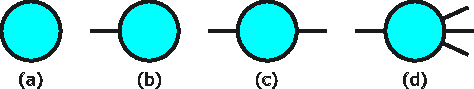
\includegraphics[width=0.5\linewidth]{tensor-example.pdf}
    \caption{Some examples of tensors. 
    (a) A scalar has no legs. 
    (b) A vector has one leg.
    (c) A matrix has two legs.
    (d) A rank-4 tensor has four legs.}
    \label{fig:tensor-example}
\end{figure}

In some contexts, the geometric shape and the direction of the legs are determined by the properties of the tensor and its indices.
When representing quantum states, the direction of the legs often indicates whether the vectors are in the Hilbert space for kets or its dual space.
Following this convention easily prevents prohibited contractions, such as a contraction between two kets.


We will now explain the five key operations in tensor networks.
First, we will explain the operations performed on a single tensor: partial trace, grouping, splitting, and singular value decomposition.
Particularly, singular value decomposition is a crucial tool for harnessing the power of tensor networks in data compression.
Then, we will explain the operations performed on multiple tensors: tensor product and contraction.
Since the primary benefit of tensor network notation lies in its ability to create networks composed of multiple tensors, this will enable the full potential of tensor networks to be realized.

% テンソル演算2: trace(TR2-4)
The first operation is the partial trace.
For a tensor $A$ with identical dimensions for the $x$-th and $y$-th indices, the partial trace is a joint summation over that index:
\begin{equation}
    \mathrm{Tr}_{x,y}(A)_{i_1,\dots,i_{x-1},i_{x+1},\dots,i_{y-1},i_{y+1},\dots,i_r}=\sum_{\alpha=1}^{d_x} A_{i_1,\dots,i_{x-1},\alpha,i_{x+1},\dots,i_{y-1},\alpha,i_{y+1},\dots,i_r},
\end{equation}
where $r$ is the rank of $A$ and $d_x$ is the dimension of $A$'s $x$-th index.
In tensor network notation, this summation is shown by the corresponding legs being connected.

\begin{figure}
    \centering
    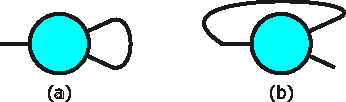
\includegraphics[width=0.4\linewidth]{fig-trace.pdf}
    \caption{Graphical examples of trace.
    When designating the left as the first axis, the upper right as the second axis, and the lower right as the third axis, (a) represents the equation $\sum_j A_{ijj}$, while (b) represents the equation $\sum_k A_{iik}$.}
    \label{fig:trace}
\end{figure}

Figure~\ref{fig:trace} gives graphical examples of trace operation in tensor network notation.
The advantage of trace notation in tensor network notation is that the summed-over indices do not need to be named.
This simplifies the notation for large networks.

One example illustrating the convenience of trace notation is the cyclic property of the trace.
As shown in Fig.~\ref{fig:trace-cyclic}, we can prove $\mathrm{Tr}(AB)=\mathrm{Tr}(BA)$ by simply sliding the tensor to change its position in the network.
Although this example is quite simple, the intuitive transformations of equations in tensor network notation become even more beneficial as the number of tensors increases.

\begin{figure}
    \centering
    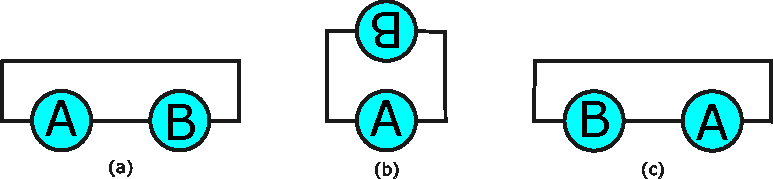
\includegraphics[width=\linewidth]{trace-cyclic.pdf}
    \caption{Diagrams illustrating the cyclic property of the trace using tensor networks. In (a), the equation $\mathrm{Tr}(AB)$ is represented in tensor network notation. Tensor network notation allows for free transformations as long as the information about which axes are connected is preserved. Thus, it can be transformed from (a) to (b) to (c). Since (c) represents the equation $\mathrm{Tr}(BA)$ in tensor network notation, the cyclic property of the trace is thereby demonstrated.}
    \label{fig:trace-cyclic}
\end{figure}

% テンソル演算4: grouping and splitting(TR2-6)
The second and third operations we explain are grouping and splitting.
The space of tensors $\mathbb C^{a_1\times a_2\times \dots \times a_n}$ and $\mathbb C^b$ are isomorphic as vector spaces whenever $a_1\times a_2\times \dots \times a_n=b$ holds.
This allows us to apply concepts and techniques previously defined for vectors and matrices to all tensors.
We can group indices to lower a tensor's rank or split them to raise it.

The definitions of grouping and splitting used in this thesis are as follows.
Just as there are various ways to convert a matrix into a vector, there are multiple ways for grouping and splitting.
We use an index convention that generalizes column-major ordering to higher dimensions.
% If we take $n$ index, we form a grouped index by
For simplicity, if we group all the indices of rank $r$ tensor $A$, the resulting grouped tensor can be written as
\begin{equation}
    A_I \coloneqq A_{i_1,\dots,i_n},
\end{equation}
where we have defined our grouped indices as
\begin{equation}
    I \coloneqq i_1 + d_1 i_2 + d_1 d_2 i_3 + \dots + (d_1 \times \cdots \times d_{n-1}) i_n ,
\end{equation}
and $d_x$ is the dimension of the $x$-th index.
According to this rule, we will refer to the process of combining indices as grouping and the process of separating indices as splitting.

In tensor network notation, grouping is represented by combining multiple indices into a single index, while splitting is represented by dividing a single index into multiple indices.
Figure~\ref{fig:grouping-splitting} depicts some examples of grouping and splitting.
The resulting grouped index is often depicted with a bold line to distinguish it from the original indices.

\begin{figure}
    \centering
    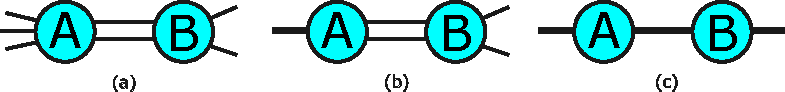
\includegraphics[width=\linewidth]{grouping-splitting.pdf}
    \caption{Graphical examples of grouping and splitting.
    By grouping the left indices in (a), we obtain (b). 
    Further grouping the central and right indices in (b) results in (c). 
    Since (c) represents a simple matrix product, the complex tensor network contraction is reduced to a matrix product. 
    Conversely, the process of decomposing from (c) to (b) and then to (a) is known as splitting.}
    \label{fig:grouping-splitting}
\end{figure}

% テンソル演算5: SVD(TR2-7)
The fourth operation we explain is the singular value decomposition~(SVD).
Any $M\times N$ matrix $A$ can be decomposed as $A=USV^\dagger$ using SVD, where $U$ is an $M\times M$ unitary matrix, $V^\dagger$ is an $N\times N $ unitary, matrix, and $S$ is a real diagonal matrix with non-negative entries.
SVD is a crucial algorithm for finding the best approximation.
If we keep the largest $k$ singular values in $S$ to form $S^{(k)}$, then $A^{(k)}=US^{(k)}V^\dagger$ is the closest rank-$k$ matrix to $A$ in the Frobenius norm.
This property is often used for dimensionality reduction while preserving as much information as possible.

SVD for matrices can be extended to general tensors using the grouping and splitting algorithm.
Let $T$ be a tensor of rank $n+m$.
By grouping $n$ indices as rows and $m$ indices as columns and then performing SVD, we get a higher dimensional version of SVD:
\begin{equation}
    T_{i_1,\dots,i_m;j_1,\dots,j_n}=\sum_\alpha U_{i_1,\dots,i_m,\alpha}S_{\alpha,\alpha} (V_{j_1,\dots,j_n,\alpha})^*,
\end{equation}
where $U$ and $V$ are isometries ($U^\dagger U=V^\dagger V=I$) across the indicated partitioning. %, the conjugation in $V^\dagger$ is included to maintain consistency with conventional notation and is also applied with respect to this partitioning.
Similar to the matrix case, if $S^{(k)}$ is the $k\times k$ matrix formed by retaining the largest $k$ singular values in $S$, then
\begin{equation}
    T_{i_1,\dots,i_m;j_1,\dots,j_n}^{(k)}=\sum_\alpha^k U_{i_1,\dots,i_m,\alpha}S_{\alpha,\alpha}^{(k)} (V_{j_1,\dots,j_n,\alpha})^*
\end{equation}
is the rank-$k$ tensor closest to $T$ in terms of the Frobenius norm.
This approach allows for dimensionality reduction in tensor networks while preserving essential information.
Figure~\ref{fig:svd} represents the diagram of SVD for tensors.
\begin{figure}
    \centering
    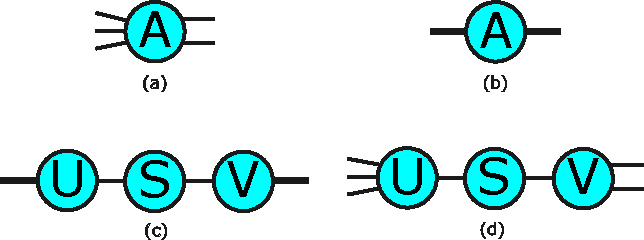
\includegraphics[width=0.7\linewidth]{fig-svd.pdf}
    \caption{Diagrams for tensor SVD.
    For a general tensor $A$ (a), by grouping the left and right axes respectively, it can be regarded as a matrix, as shown in (b). 
    Applying SVD to the matrix results in its decomposition into unitary matrices $U$ and $V$ and a diagonal matrix $S$ containing the singular values (c). 
    By splitting indices, the SVD of the tensor is obtained while preserving the original tensor's axis information (d).}
    \label{fig:svd}
\end{figure}

% テンソル演算1: tensor product(TR2-3)
Next, we consider operations involving multiple tensors.
The fifth operation is the tensor product, which is a generalization of the outer product of vectors.
The tensor product's value for a given set of indices is the element-wise product of the constituent tensor's values.
Explicitly expressed in index notation, the binary tensor product takes the form:
\begin{equation}
    [A\otimes B]_{i_1,\dots,i_r,j_1,\dots,j_s}\coloneqq A_{i_1,\dots,i_r}\cdot B_{j_1,\dots,j_s}.
\end{equation}
Diagrammatically, the tensor product is represented by placing two tensors adjacent, as shown in Fig.~\ref{fig:tensor-product}.
Therefore, the value of a network with disjoint tensors is simply the product of their values.
\begin{figure}
    \centering
    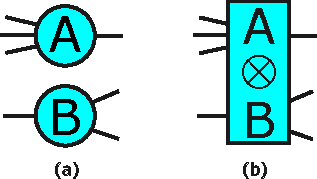
\includegraphics[width=0.4\linewidth]{tensor-product.pdf}
    \caption{Diagrams representing the tensor product of two tensors.
    As shown in (a), two unconnected tensors are combined using the tensor product. 
    This can also be explicitly denoted as a tensor product, as illustrated in (b).}
    \label{fig:tensor-product}
\end{figure}

% テンソル演算3: contraction(TR2-5)
The most frequently utilized operation is contraction, a tensor product followed by a trace over the indices of two tensors.
The contraction of $A$'s $x$-th index and $B$'s $y$-th index is defined as
\begin{equation}
    C_{i_1,\dots,i_{x-1},i_{x+1},\dots,i_r,j_1,j_{y-1},j_{y+1},\dots,j_s}=\sum_\alpha A_{i_1,\dots,i_{x-1},\alpha,i_{x+1},i_r}B_{j_1,\dots,j_{y-1},\alpha,j_{y+1},\dots,j_s},
\end{equation}
where $C$ is the result of the contraction.
The inner product of vectors, matrix-vector multiplications, and matrix-matrix multiplications are all contractions, as in Fig.~\ref{fig:contraction}.
\begin{figure}
    \centering
    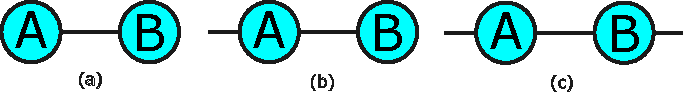
\includegraphics[width=0.8\linewidth]{fig-contraction.pdf}
    \caption{Some examples of the contraction.
    In (a), we observe the dot product of vectors, in (b), the product of a matrix and a vector, and in (c), the matrix product. 
    Each of these represents a well-known special case of contraction.}
    \label{fig:contraction}
\end{figure}


% テンソルネットワークの定義(TR2-8)
By integrating the aforementioned tensor operations, we can define a tensor network as a diagram that specifies how to combine multiple tensors into a single composite tensor.
The rank of this tensor is determined by the number of unmatched legs in the diagram.
The value for a given set of external indices is the product of the constituent tensor's values, summed over all internal index labelings consistent with the contractions.

% 縮約の順番,Bubbling(TR2-9)
Although tensor networks are designed so their values do not depend on the order of tensor contractions, the sequence affects computational complexity and practicality.
One can contract tensor networks by starting with one tensor and sequentially contracting it with others.
This sequence, called bubbling, continues until the network is fully absorbed into the stored tensor, leaving only the final result.
Many networks can be bubbled efficiently or inefficiently.
We need to be careful when arranging the order of contractions.

% MPSの内積に関する例
As an example of how the order of contractions can significantly affect computational complexity, consider the bubbling of a ladder-shaped network that appears in calculations, such as the inner product of MPSs.
One approach is to contract along the top of the ladder, then back along the bottom, illustrated in Fig.~\ref{fig:bubbling1}.
This method is inefficient since, for a ladder of length $n$, the tensor tracked at the midpoint has rank $n$, causing the number of entries to scale exponentially.
As a result, the memory and time needed for this contraction are exponential, making it impractical for large $n$.
However, by contracting each rung in sequence, the tracked tensor's rank stays at three or below, leading to constant memory and linear time costs depicted in Fig.~\ref{fig:bubbling2}.
\begin{figure}
    \centering
    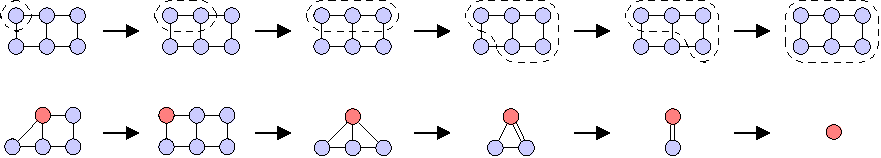
\includegraphics[width=\linewidth]{fig-bubbling1.pdf}
    \caption{An example of inefficient bubbling in a ladder-shaped network.
    In this example, the contraction proceeds sequentially from the tensors in the upper row. 
    However, the spatial computational complexity increases exponentially with the ladder length at the intermediate point. 
    Consequently, for long ladders, current computers are unable to complete the contraction calculations.}
    \label{fig:bubbling1}
\end{figure}
\begin{figure}
    \centering
    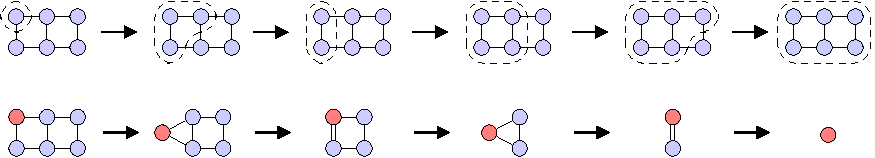
\includegraphics[width=\linewidth]{fig-bubbling2.pdf}
    \caption{An example of efficient bubbling in a ladder-shaped network.
    For a ladder-shaped network, as in this example, sequentially contracting from the left achieves a computational complexity that is linear with respect to the ladder length.}
    \label{fig:bubbling2}
\end{figure}



Although our example shows bubbling where one tensor contracts others one by one, this is not always the most efficient method; a multi-bubbling approach is often faster.
It is crucial to determine the appropriate grouping of parts, the starting tensor, and the contraction sequence to reduce computational complexity.

% \subsection{Advantages of using tensor networks}
% テンソルネットワークの長所はEfficient data representationであること

% 高次元のデータを扱う様々な分野に応用されていること

% 量子状態も高次元であり古典での愚直なシミュレートが困難

% テンソルネットワークを用いることでシミュレートできる

\begin{figure}
    \centering
    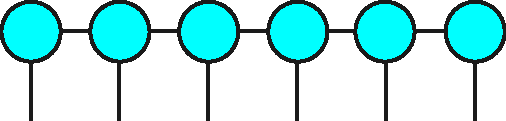
\includegraphics[width=0.5\linewidth]{mps.pdf}
    \caption{MPS represented in tensor network notation, specifically for a system size of six.}
    \label{fig:mps}
\end{figure}
\begin{figure}
    \centering
    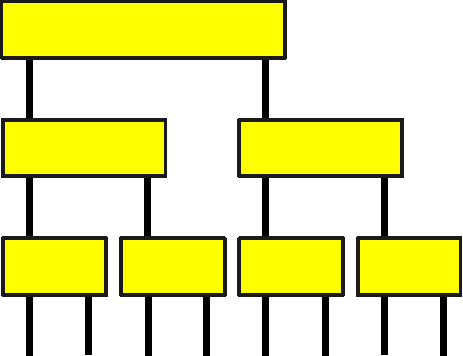
\includegraphics[width=0.5\linewidth]{ttn.pdf}
    \caption{TTN represented in tensor network notation, specifically for a binary tree with a system size of eight.}
    \label{fig:ttn}
\end{figure}

% \begin{figure}
%     \centering
%     \begin{minipage}[b]{0.45\linewidth}
%         \centering
%         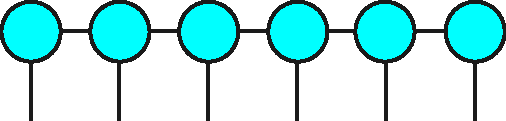
\includegraphics[width=\linewidth]{mps.pdf}
%         \caption{An MPS represented in tensor network notation, specifically for a system size of six.}
%         \label{fig:mps}
%     \end{minipage}
%     \hspace{0.05\linewidth}
%     \begin{minipage}[b]{0.45\linewidth}
%         \centering
%         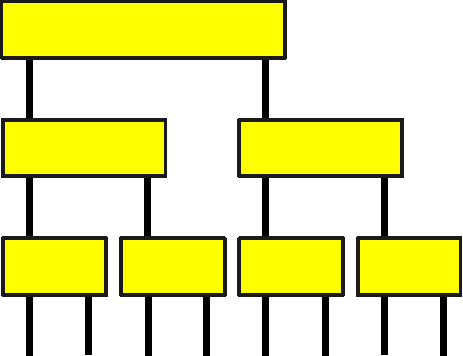
\includegraphics[width=\linewidth]{ttn.pdf}
%         \caption{A TTN represented in tensor network notation, specifically for a binary tree with a system size of eight.}
%         \label{fig:ttn}
%     \end{minipage}
% \end{figure}
\section{MPSs and TTNs}
As illustrated in Fig.~\ref{fig:mps}, Matrix Product States~(MPSs) represent the simplest form of tensor networks, with tensors arranged in a single line. 
Advanced algorithms such as Density Matrix Renormalization Group~(DMRG) and Time-Evolving Block Decimation~(TEBD) have been developed, facilitating their application across various fields. 
In contrast, Tree Tensor Networks~(TTNs), depicted in Fig.~\ref{fig:ttn}, have a more complex tree-like structure.
It is evident that MPSs can be considered a subset of TTNs.
One notable advantage of TTNs is that the distance between any pair of leaf nodes scales logarithmically with the number of nodes, in contrast to the linear scaling observed in MPSs. 
Since connected correlation functions in tensor networks typically decay exponentially with path length, TTNs are inherently more effective at capturing long-range correlations and are particularly well-suited for representing two-dimensional systems. 
As a result, TTNs have found applications in diverse domains, including quantum chemistry~\cite{chemical1,chemical2}, condensed matter physics~\cite{condmat1,condmat2,condmat3}, and machine learning~\cite{ml1,ml2}.

Let $\ket{\psi}$ be a tensor network in the form of either an MPS or a TTN.
Number the tensors in $\ket{\psi}$ from left to right for MPS, and in breadth-first search~(BFS) order from the root node for TTN, denoting the $i$-th tensor as $A^{(i)} (i=1,\dots,N)$.
By adding a leg with bond dimension one, a two-legged tensor can be converted into a three-legged tensor, thus all tensors in $\ket{\psi}$ can be considered three-legged.
$\ket{\psi}$ is in canonical form if there exists a node $A^{(i)}$, called the canonical center, such that for all other nodes $A^{(i')}$ the following holds
\begin{equation}
    \sum_{l,m}A^{(i')}_{l,m,n}A^{(i')*}_{l,m,n'}=I_{n,n'},
\end{equation}
where the leg denoted by index $n$ is the unique leg of $A^{(i')}$ pointing towards $A^{(i)}$.
A tensor that satisfies this equation is referred to as an isometric tensor.
Any $\ket{\psi}$ can be transformed into this canonical form, and the position of the canonical center can be freely moved without changing the quantum state.

The canonical form offers numerous advantages.
In this thesis, the key benefit is that at the canonical center, the local SVD becomes equivalent to the global SVD, allowing for precise bond dimension reduction through truncation while appropriately moving the canonical center.
Additionally, in the canonical form, each tensor is an isometry, facilitating easy conversion to unitary form and embedding into quantum circuits. 
Unless otherwise specified, we assume that any MPSs and TTNs are converted to the canonical form with $A^{(0)}$ as the canonical center.

\section{Embedding of MPSs}
% \begin{figure}
%     \centering
%     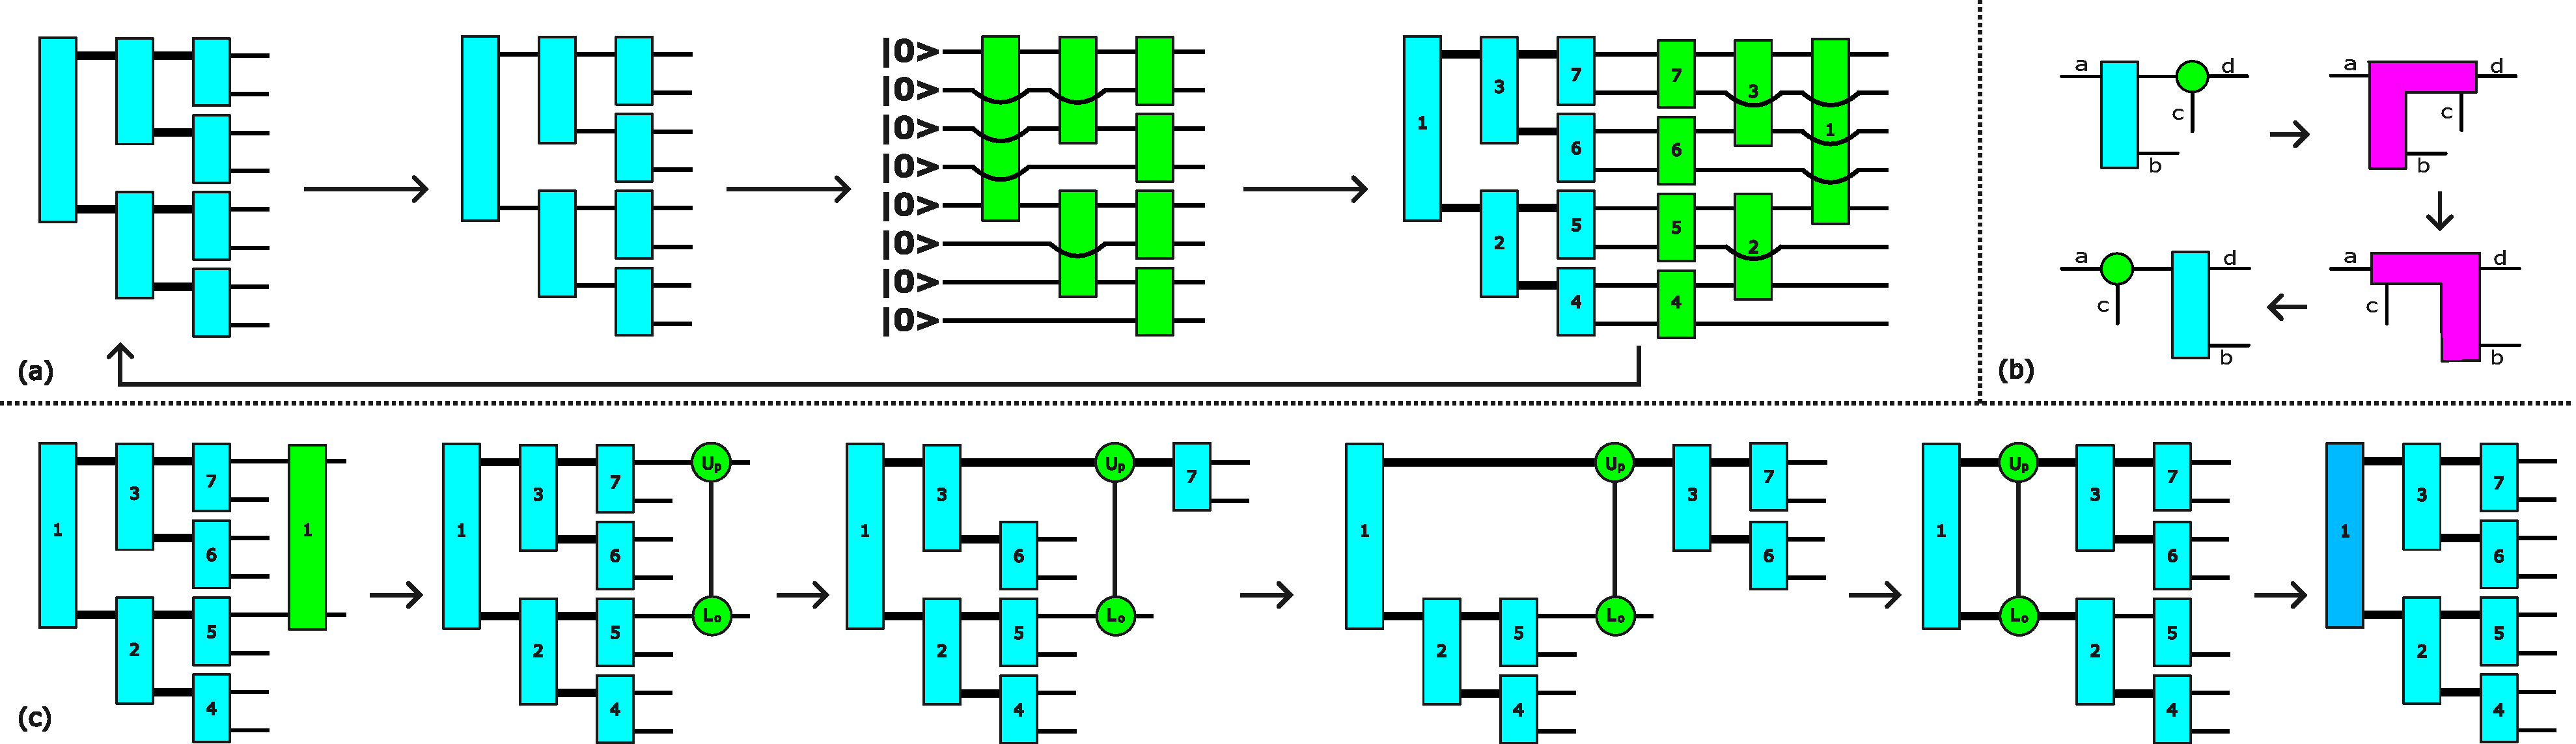
\includegraphics[width=\linewidth]{fig-decomposition.pdf}
%     \caption{A schematic diagram illustrating the analytical decomposition for a TTN. (a) The TTN is truncated to a bond dimension of two using SVD. This simplified TTN is then embedded into a quantum circuit by converting tensors into unitaries via Gram-Schmidt orthogonalization. These unitaries act as disentanglers and are applied to the original TTN. By repeating these steps, a multi-layer quantum circuit is formed. (b) A diagram of a penetration algorithm. It contracts two connected tensors, reorders axes, and separates them using SVD, making it seem like their positions have swapped. (c) A schematic diagram explaining the transformation from a complex tensor network into a TTN. We number the tensors based on their positions in the network. We first use SVD to split it into an upper and a lower tensor. Then, we apply the penetration algorithm iteratively until the upper tensor is connected with the corresponding tensor. This process is repeated for the lower tensor as well. Finally, we contract the upper and lower tensors with the corresponding tensor to form a new tensor in the TTN. This process is performed sequentially from the highest-numbered component of the disentangler.}
%     \label{fig:decomposition}
% \end{figure}





% \begin{figure*}[!h]
%   \centering
%    {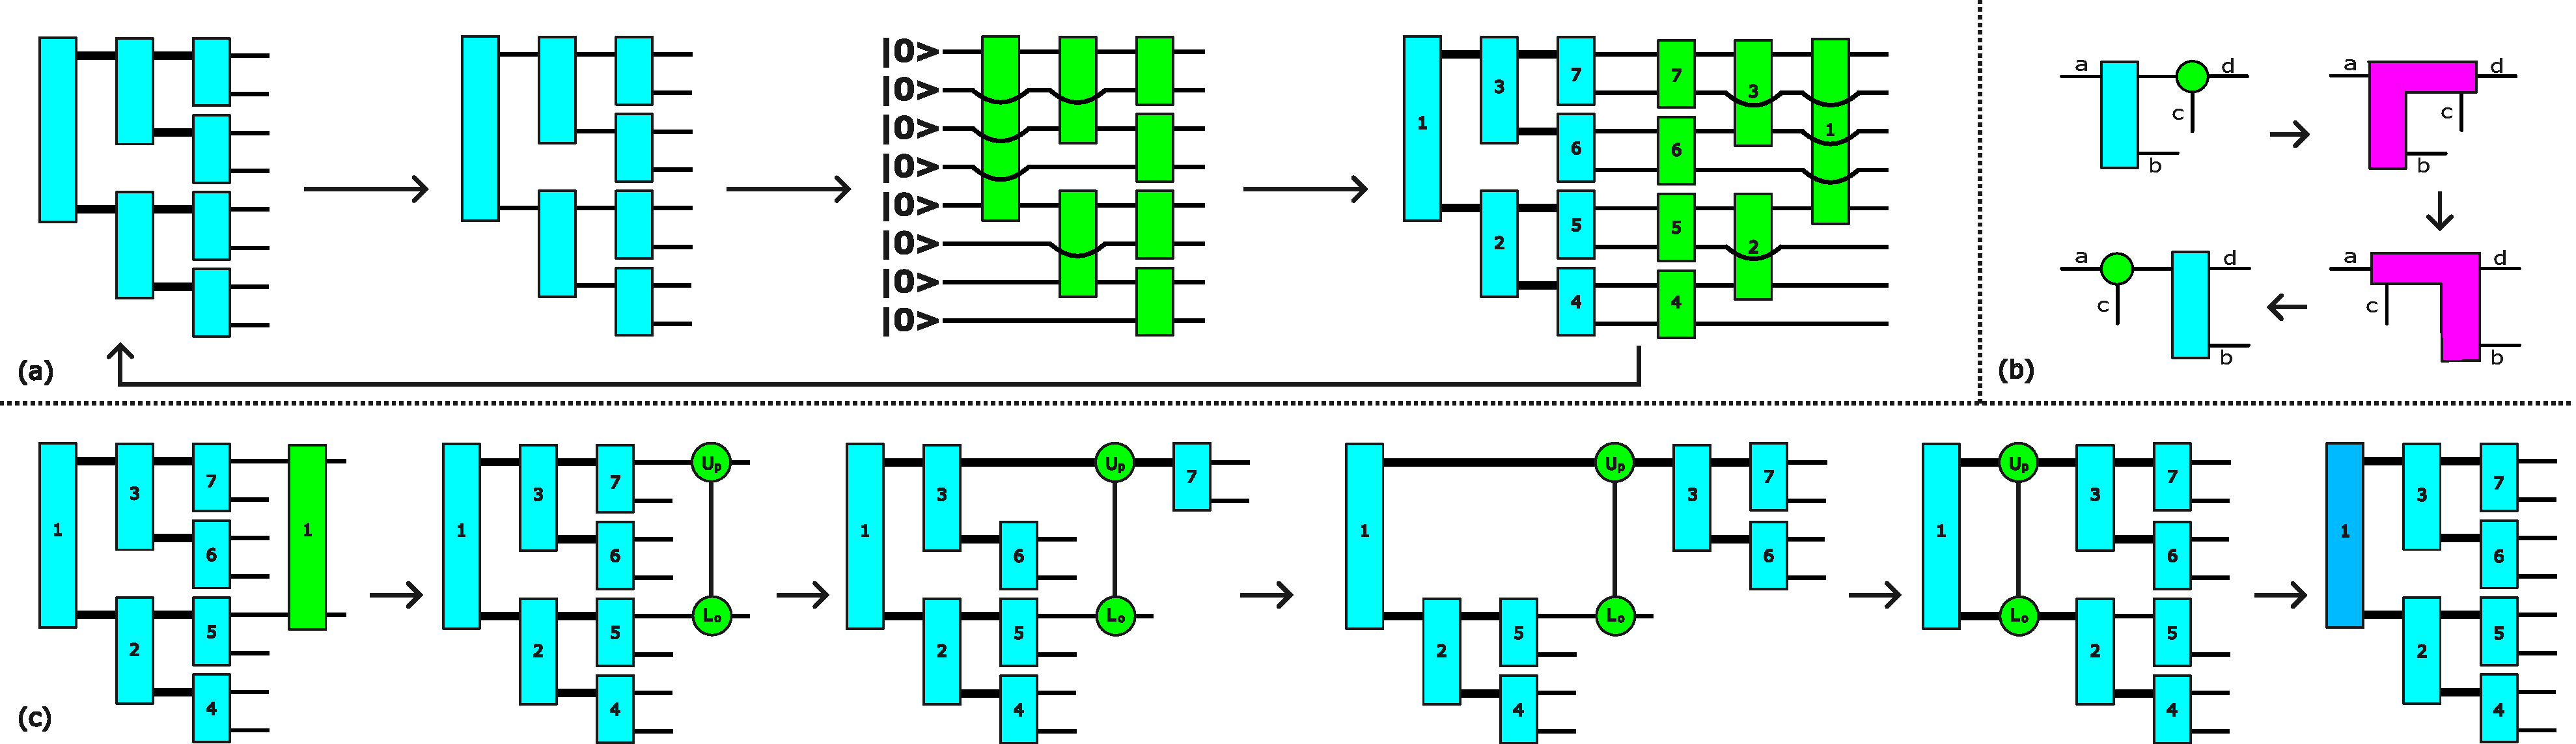
\epsfig{file = fig-decomposition.pdf, width = 15cm}}
%   \caption{A schematic diagram illustrating the analytical decomposition for a TTN. (a) The TTN is truncated to a bond dimension of two using SVD. This simplified TTN is then embedded into a quantum circuit by converting tensors into unitaries via Gram-Schmidt orthogonalization. These unitaries act as disentanglers and are applied to the original TTN. By repeating these steps, a multi-layer quantum circuit is formed. (b) A diagram of a penetration algorithm. It contracts two connected tensors, reorders axes, and separates them using SVD, making it seem like their positions have swapped. (c) A schematic diagram explaining the transformation from a complex tensor network into a TTN. We number the tensors based on their positions in the network. We first use SVD to split it into an upper and a lower tensor. Then, we apply the penetration algorithm iteratively until the upper tensor is connected with the corresponding tensor. This process is repeated for the lower tensor as well. Finally, we contract the upper and lower tensors with the corresponding tensor to form a new tensor in the TTN. This process is performed sequentially from the highest-numbered component of the disentangler.}
%   \label{fig:decomposition}
%  \end{figure*}
 
Although embedding general tensor networks into shallow quantum circuits is challenging, several workable methods have been proposed for MPSs.
In this subsection, we overview the technique for seamlessly embedding MPSs into shallow quantum circuits.

% analytical decomposition by disentangling
\cite{EncodingMPS} introduced an analytical decomposition method for an MPS into several layers of two-qubit gates with a linear next-neighbor topology. 
First, the MPS $\ket{\psi^{(k)}}$ with bond dimension $\chi$ is truncated to a bond dimension two MPS $\ket{\psi_{\chi=2}^{(k)}}$.
Next, the isometric tensors in $\ket{\psi_{\chi=2}^{(k)}}$ are converted into unitary tensors.
The resulting set of unitary tensors, $L[U]^{(k)}$, is referred to as a layer and can be embedded into a quantum circuit composed of two-qubit gates.
Additionally, since
\begin{equation}
    \ket{\psi_{\chi=2}^{(k)}}=\mathrm{L}[U]^{(k)}\ket{0}
\end{equation}
and
\begin{equation}
    \mathrm{L}[U]^{(k)\dagger}\ket{\psi_{\chi=2}^{(k)}}=\ket{0}
\end{equation}
are holds, $L[U]^{(k)\dagger}$ can be considered a disentangler, transforming the quantum state into a product state.
Finally, a new MPS $\ket{\psi^{(k+1)}}=\mathrm{L}[U]^{(k)\dagger}\ket{\psi^{(k)}}$ can be obtained.
Since $L[U]^{(k)\dagger}$ acts as a disentangler, $\ket{\psi^{(k+1)}}$ should have reduced entanglement compared to $\ket{\psi^{(k)}}$.
By repeating this process starting from the original MPS $\ket{\psi^{(0)}}$, a quantum circuit $\prod_{k=1}^K \mathrm{L}[U]^{(k)}\ket{0}$ with multiple layers can be generated.
 
% decomposition by optimization
Optimization-based methods are employed as an alternative approach to embedding tensor networks into quantum circuits.
This method sequentially optimizes the unitary operators within the quantum circuit to maximize the magnitude of the inner product between the quantum circuit and the tensor network.
\cite{env-tensor} proposed an iterative optimization technique that utilizes the calculation of environment tensors and SVD.
Similarly, \cite{mpsoptim} employed this iterative optimization method to embed quantum states into quantum circuits.
An environment tensor is calculated to update a unitary by removing the unitary from the circuit and contracting the remaining tensor network.
This tensor represents the optimal operator for increasing fidelity, though it is not inherently unitary.
To ensure unitarity, an SVD is performed, and the resulting product is used to find the unitary matrix that best approximates the optimal operator.
For a more detailed explanation of the optimization algorithm, please refer to \cite{mpsdecomp} or the chapter on optimization algorithms for TTNs described later.


% decomposition of MPS
\cite{mpsdecomp} investigated the optimal sequence for combining these two methods to achieve the highest accuracy.
The study concludes that the best results are obtained by adding new layers through an analytical decomposition step and optimizing all layers with each addition.
This method has achieved exceptional accuracy in embedding a wide range of MPSs in fields such as physics, machine learning, and random systems.
Therefore, it can be considered one of the best current techniques for embedding MPSs into shallow circuits.
However, this method does not support embedding tensor networks other than MPSs.
Consequently, embedding tensor networks such as TTNs and other non-MPS structures remains an unresolved issue.

% \section{Matrix Product States}
% \subsection{Introduction to matrix product states}
% 一般のテンソルからMPSへの変換方法

% virtual indexやbond indexなど用語の説明

% ボンド次元とエンタングルメントエントロピーの関係

% MPSの例
%% Product, W, GHZ, AKLT state

% MPSの性質: カノニカル形式への変換

% ほとんどの基底状態はMPSで表現できること

% MPSの課題: 相関が長い系は表現できない


% \subsection{Density Matrix Renormalization Group}
% MPSは非常に精度良く基底状態を求めるアルゴリズムが知られていること

% DMRGの手法の詳細


% \section{Tree Tenser Networks}
% 一般のテンソルからTTNへの変換方法

% TTNの基本用語の説明

% MPSと同様の利点

% MPSと比べて相関が長い系の表現に適している理由

% 具体的な応用例

% \section{Compatibility with quantum circuits}
% 任意の量子回路はテンソルネットワークで表現できること


% テンソルネットワークは近似的に量子回路に埋め込めること


% PQCのパラメータをテンソルネットワークで初期化するのは自然な発想であること

% テンソルネットワークを浅い量子回路に埋め込むのは一般に難しいこと
% \cleardoublepage
% \chapter{Embedding of MPS to shallow quantum circuits}
% MPSを使ってPQCを初期化するモチベを再度まとめる

% 取り組む問題を定式化しておく(入力, 出力など)

% \section{methods}


% \subsection{Analytic decomposition by disentangling}

% MPSを1レイヤーに埋め込む概要(EM4)

% MPDの定義(EM5)

% MPDの構成方法1: 最後のテンソルはそのまま1qubit-gateに変換できること(EM5)

% MPDの構成方法2: 中間のテンソルの作り方(EM6)

% MPDの構成方法3: 最初のテンソルの作り方(EM7)

% このように構成したMPDがMPDの条件を満たしていること(EM7)

% MPSを複数のレイヤーに埋め込む概要(EM11)

% 評価指標(Fidelity)の説明(DMA1)

% MPSを複数のレイヤーに埋め込むアルゴリズムの流れ(EM11, DMA2)

% アルゴリズムの説明(DMA3)

% このアルゴリズムの長所と短所(DMA4)
% \subsection{Decomposition by optimization}
% optimizationアルゴリズムの概要(DMB1)

% アルゴリズムの流れ(DMB2)

% アルゴリズムの説明(DMB3)

% このアルゴリズムの長所と短所(DMB5)


% Combinationを考えるモチベーションと概要(DMC1)

% decomposition, optimizationそれぞれの長所短所を踏まえた将来的なモチベーション(DMC2)

% Fig3の説明(DMC3)

% 組み合わせ方の説明(DMC4)

% 最適な組み合わせ方(DMC5)

% \subsection{Computational complexity}
% 計算量を考えることの大切さ(DMD1)

% カノニカル形式にする際の計算量(DMD2)

% それぞれの組み合わせアルゴリズムの計算量(DMD3)



% \section{Results and Discussions}
% 先行研究の実験の概要

% 先行研究で使われているMPS1: 2次元ハイゼンベルグの説明

% 先行研究で使われているMPS2: BASデータセットの説明

% 先行研究で使われているMPS3: Random MPSの説明

% fig4の説明

% D_i, O_allが最も良いという結果

% 先行研究の課題1: mps以外のテンソルネットワーク構造には対応していないこと

% 先行研究の課題2: disentanglerを作用させてもエンタングルメントが減少するとは限らないこと

%% 1に収束していないという結果の説明

%% 収束精度が悪い原因としてdisentanglerでランダムベクトルをかけてしまっている点を指摘

\cleardoublepage
\chapter{Embedding of TTNs to shallow quantum circuits}
% TTNを使ってPQCを初期化するモチベを再度まとめる(TTNの方がMPSより適している理由, 浅い回路に埋め込む既存手法はないこと)

% 取り組む問題を定式化しておく
In this section, we propose a method for embedding TTNs into shallow quantum circuits.
The proposed method can be generalized to embed TTNs of any shape since any shape of TTN can be converted into a binary tree using SVD.
Below, we assume a binary tree for simplicity.
The fundamental approach of the proposed method is similar to that of MPSs~\cite{mpsdecomp}. 
By repeatedly adding layers using the analytical decomposition algorithm and optimizing the entire circuit, we generate highly accurate embedded quantum circuits.
This chapter first introduces the analytical decomposition algorithm for TTNs.
Due to the increased structural complexity of TTNs compared to MPSs, the contraction methods become non-trivial. 
We propose a method that balances approximation error and computational cost.
Next, we describe the optimization algorithm for TTNs and integrate it with the analytical decomposition.
Finally, we discuss the computational cost and demonstrate that embedding TTNs is feasible within practical computational limits.

\section{Overview of this method}


\subsection{Analytic decomposition by disentangling}
Our analytical decomposition algorithm for TTNs is an extension of the algorithm for MPSs introduced in \cite{EncodingMPS}.
We denote the original TTN as $\ket{\psi_0}$, the $k$-th layer of the quantum circuit as $\mathrm{L}[U]^{(k)}$, the number of layers in resulting quantum circuit as $K$, and the resulting quantum circuit as $\prod_{k=1}^K \mathrm{L}[U]^{(k)}\ket{0}$.
Algorithm~\ref{algorithm:decomposition} details the analytical decomposition process for TTNs, as depicted in Fig.~\ref{fig:decomposition-a}.

\begin{figure}
    \centering
    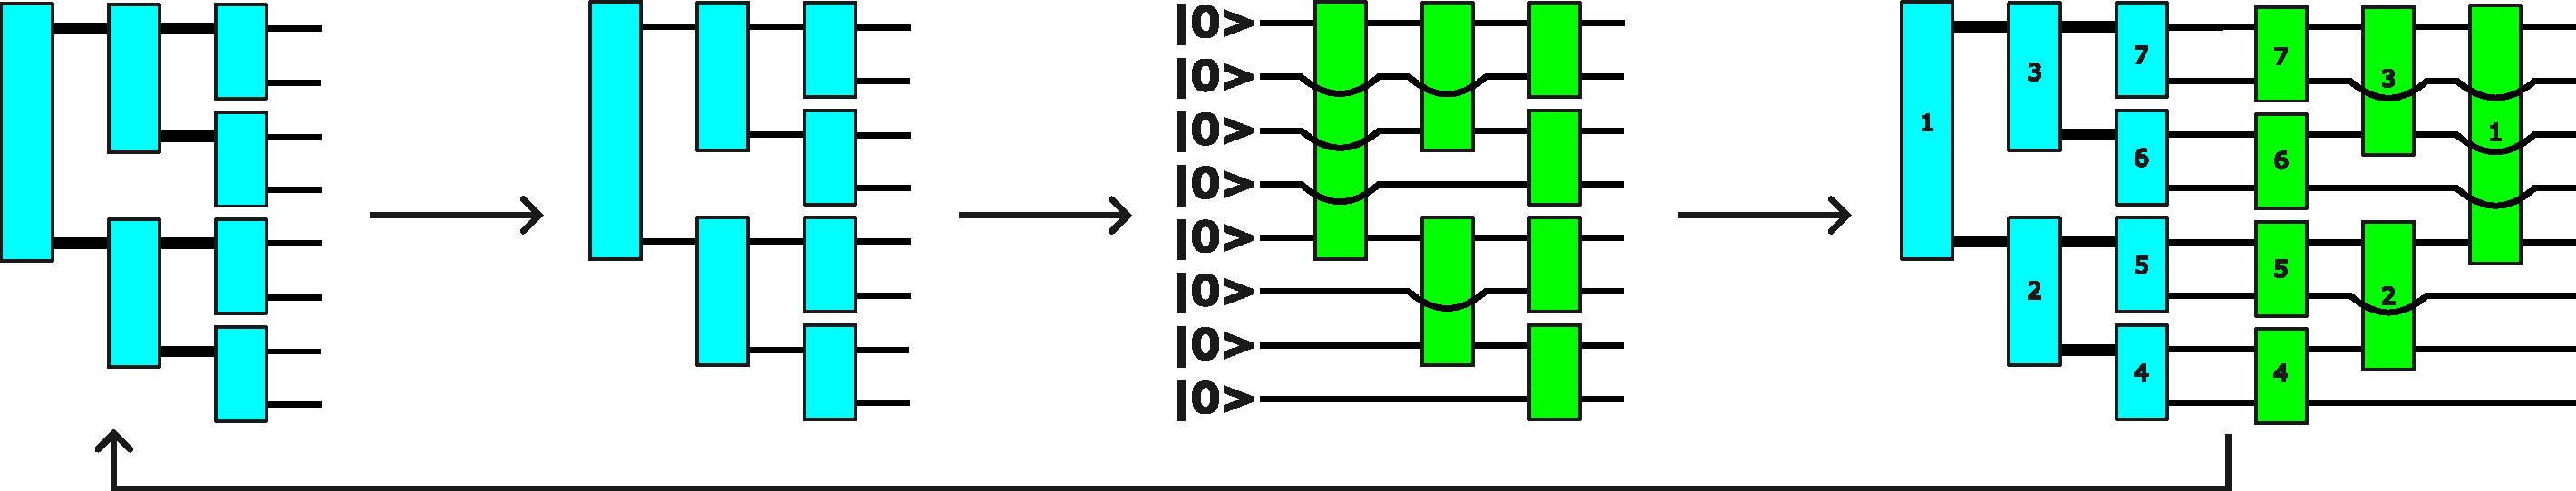
\includegraphics[width=\linewidth]{fig-decomposition-a.pdf}
    \caption{A schematic diagram illustrating the analytical decomposition for a TTN.
    The TTN is truncated to a bond dimension of two using SVD. This simplified TTN is then embedded into a quantum circuit by converting tensors into unitaries via Gram-Schmidt orthogonalization. These unitaries act as disentanglers and are applied to the original TTN. By repeating these steps, a multi-layer quantum circuit is formed.
    }
    \label{fig:decomposition-a}
\end{figure}

\begin{algorithm}[tbp]
 \caption{Analytical decomposition of TTN.}
 \label{algorithm:decomposition}
 \KwIn{TTN $\ket{\psi_0}$, Maximum number of layers $K$}
 \KwOut{Quantum Circuit $\prod_{k=1}^K \mathrm{L}[U]^{(k)}\ket{0}$}
 $\ket{\psi^{(1)}} \leftarrow{\ket{\psi_0}}$\;
 \For{$k=1$ to $K$}{
 Truncate $\ket{\psi^{(k)}}$ to $\ket{\psi^{(k)}_{\chi=2}}$ via SVD\;
 Convert $\ket{\psi^{(k)}_{\chi=2}}$ to $\mathrm{L}[U]^{(k)}$\;
 $\ket{\psi^{(k+1)}} \leftarrow{\mathrm{L}[U]^{(k)\dagger}}\ket{\psi^{(k)}}$\;
 }
\end{algorithm}

In this algorithm, a copy of the original TTN is truncated to a lower dimension using SVD.
Converting a TTN with bond dimension $\chi$ to bond dimension two can be done accurately, similar to MPSs, by shifting the canonical center so that the local SVD matches the global SVD.
This truncated TTN is then transformed into a single layer of two-qubit gates by converting the isometric tensors in the layer into unitary tensors using the Gram-Schmidt orthogonalization process.
 The inverse of this layer is applied to the original TTN, resulting in a partially disentangled state with potentially reduced entanglement and bond dimensions.
This process can be iteratively repeated to generate multiple layers, which are indexed in reverse order to form a circuit that approximates the target TTN. 
Notably, the final layer of the disentangling circuit is used as the initial layer of the quantum circuit for approximation.

While this algorithm appears to function effectively at first glance, the computation of $\ket{\psi^{(k+1)}} \leftarrow{\mathrm{L}[U]^{(k)\dagger}}\ket{\psi^{(k)}}$ is exceedingly challenging from the perspective of tensor networks.
The structure of $\ket{\psi^{(k+1)}}$ is TTN, whereas tensor network $\mathrm{L}[U]^{(k)\dagger}\ket{\psi^{(k)}}$ has a more complex structure, necessitating its transformation into the shape of TTN.
As previously mentioned, the naive transformation of a general tensor network requires exponentially large memory relative to the number of qubits.
Additionally, although limiting the bond dimension during the transformation can facilitate the process, the sequence of transformations can lead to substantial approximation errors.

\begin{figure}
    \centering
    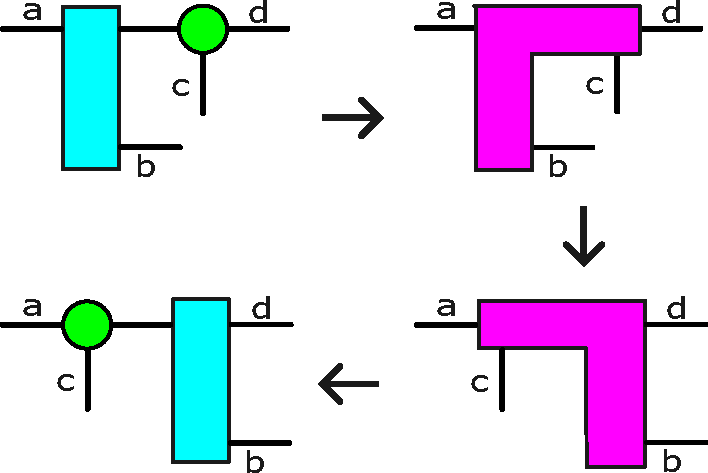
\includegraphics[width=0.6\linewidth]{fig-decomposition-b.pdf}
    \caption{Diagrams of the penetration algorithm. It contracts two connected tensors, reorders axes, and separates them using SVD, making it seem like their positions have swapped.
    }
    \label{fig:decomposition-b}
\end{figure}

To address the issue of tensor network transformations arising from the complexity of TTN structures, we propose a penetration algorithm as a submodule.
As illustrated in Fig.~\ref{fig:decomposition-b}, the penetration algorithm operates by contracting two tensors connected by a single edge along the connected axis, appropriately reordering the axes, and then separating them using SVD.
This makes it appear as if the positions of the two tensors have been swapped.
Additionally, by adjusting the number of singular values retained during SVD, we can balance the approximation accuracy and the computational cost.

\begin{algorithm}[tbp]
 \caption{Transformation of tensor networks using the penetration algorithm.}
 \label{algorithm:transformation}
 \KwIn{$\mathrm{L}[U]^{(k)\dagger}\ket{\psi^{(k)}}$}
 \KwOut{TTN $\ket{\psi^{(k+1)}}$}
 \For{$i=N-1$ to $1$}{
 Split $\mathrm{L}[U]^{(k)\dagger}_i$ into $U_p$ and $L_o$ via SVD\;
 \While{$U_p$ is not connected to $A^{(i)}$}{
 $A \leftarrow$  $U_p$'s left tensor\;
 Make $U_p$ penetrate $A$\;
 }
 \While{$L_o$ is not conntected to $A^{(i)}$}{
 $A \leftarrow$  $L_o$'s left tensor\;
 Make $L_o$ penetrate $A$\;
 }
 $A^{(i)} \leftarrow$ Contract $A^{(i)}$, $U_p$, and $L_o$\;
 }
\end{algorithm}

Algorithm~\ref{algorithm:transformation} details the transformation of tensor networks using the penetration algorithm, as depicted in Fig.~\ref{fig:decomposition-c}.
\begin{figure}
    \centering
    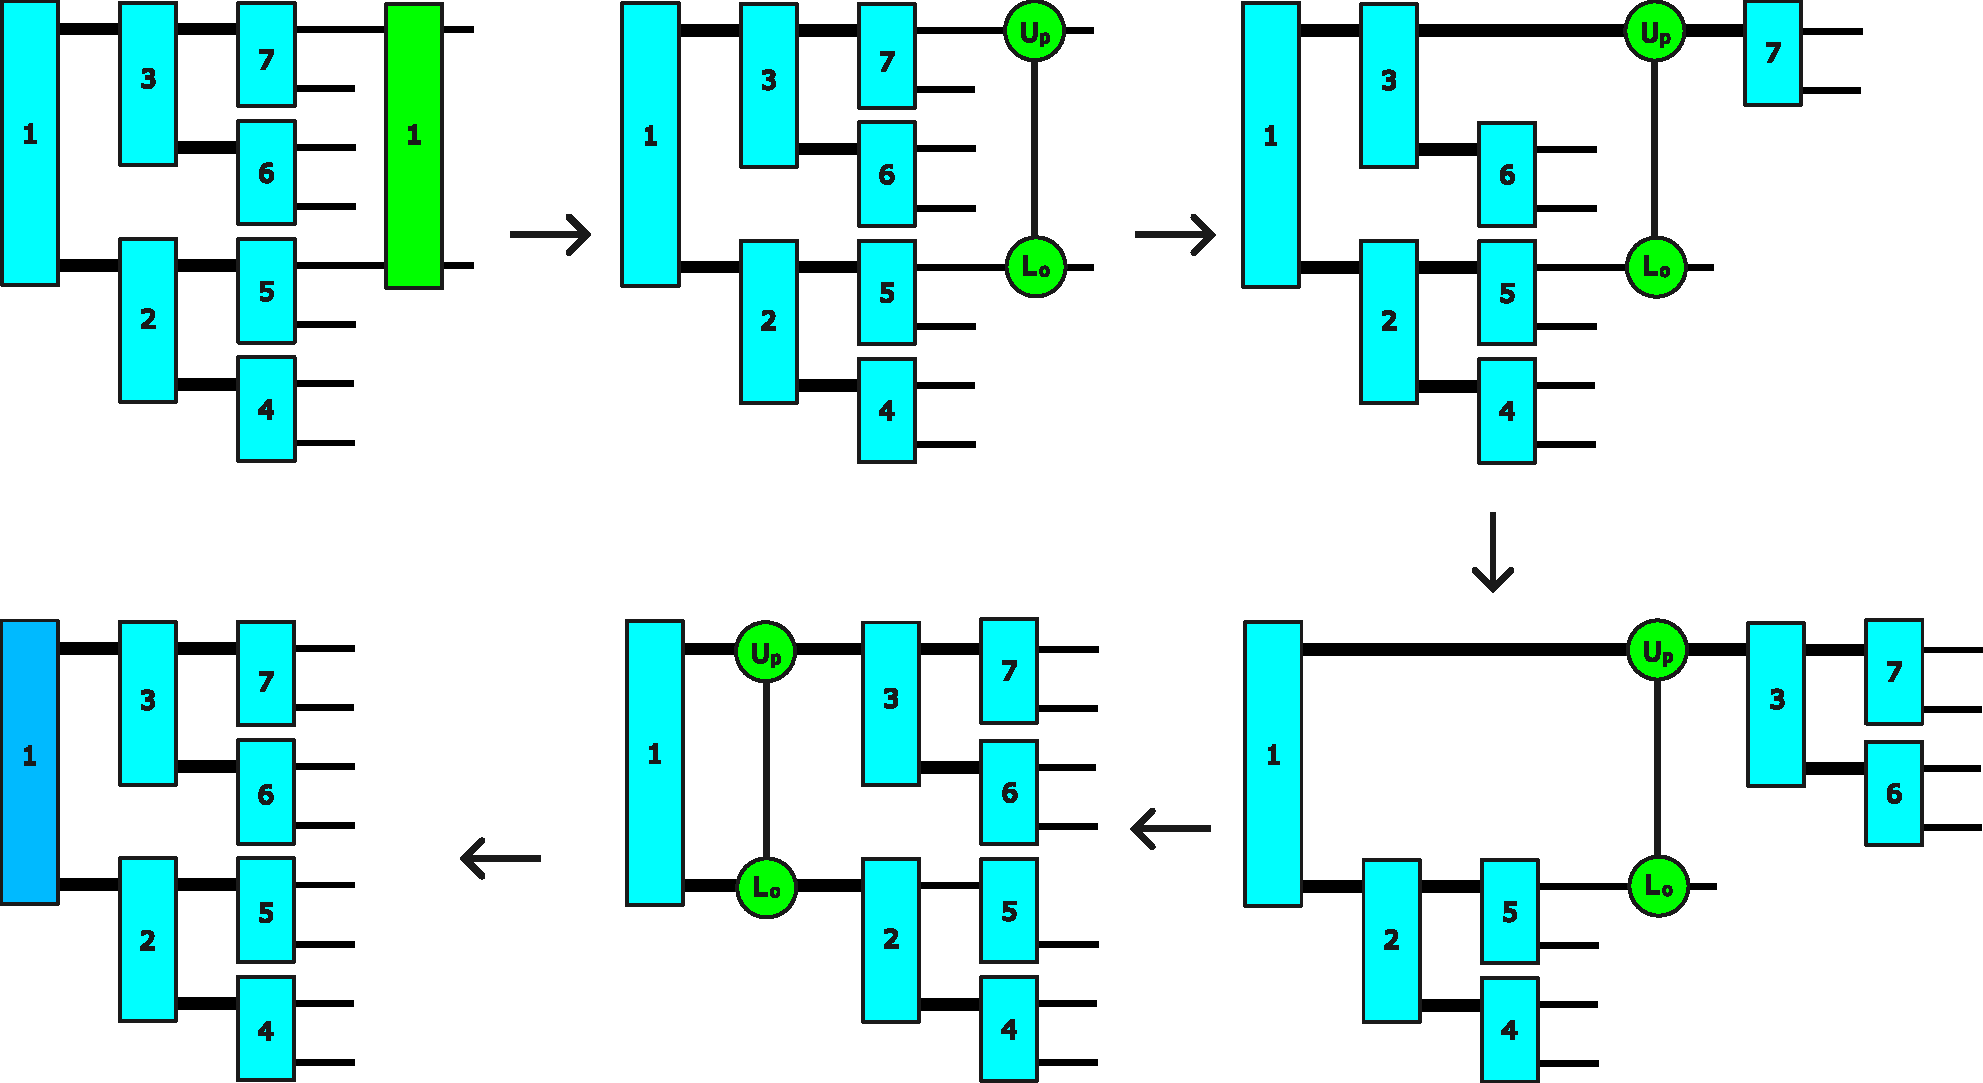
\includegraphics[width=\linewidth]{fig-decomposition-c.pdf}
    \caption{A schematic diagram explaining the transformation from a complex tensor network into a TTN. We number the tensors based on their positions in the network. We first use SVD to split it into an upper and a lower tensor. Then, we apply the penetration algorithm iteratively until the upper tensor is connected with the corresponding tensor. This process is repeated for the lower tensor as well. Finally, we contract the upper and lower tensors with the corresponding tensor to form a new tensor in the TTN. This process is performed sequentially from the highest-numbered component of the disentangler.
    }
    \label{fig:decomposition-c}
\end{figure}
We denote $i$-th tensor of $\ket{\psi^{(k)}}$ as $A^{(i)}$, where the numbers are assiend to $\ket{\psi^{(k)}}$ in breadth-first search~(BFS) order from the root.
We also assign numbers to $\mathrm{L}[U]^{(k)\dagger}$ based on its origin in the TTN, denoting the tensor with number $i$ as $\mathrm{L}[U]^{(k)\dagger}_i$.
For each tensor $\mathrm{L}[U]^{(k)\dagger}_i$ in $\mathrm{L}[U]^{(k)\dagger}$, first use SVD to split it into upper tensor $U_p$ and lower tensor $L_o$ to reduce the computational complexity in the penetration algorithm.
Then, apply the penetration algorithm iteratively until the upper tensor is connected with $A^{(i)}$.
Repeat this for the lower tensor, too.
Finally, contract the upper and lower tensors with $A^{(i)}$ to form a new TTN's $i$-th tensor.
Perform this process sequentially from the highest-numbered tensor in $\mathrm{L}[U]^{(k)\dagger}$.
This algorithm allows contraction with each tensor in $\mathrm{L}[U]^{(k)\dagger}$ without changing the TTN structure of $\ket{\psi^{(k)}}$.
Consequently, despite minor approximation errors during penetration, $\mathrm{L}[U]^{(k)\dagger}\ket{\psi^{(k)}}$ can be transformed into a TTN structure $\ket{\psi^{(k+1)}}$.

\subsection{Combination of analytic decomposition and optimization}
As demonstrated in ~\cite{mpsdecomp}, the analytical decomposition algorithm achieves the highest embedding accuracy when appropriately combined with the optimization algorithm.
In this study, we also integrate analytical decomposition with the optimization algorithm.
The fundamental concept of the optimization algorithm for quantum circuits embedded with TTNs is analogous to that for quantum circuits embedded with MPS. 
\begin{algorithm}[tbp]
 \caption{Optimization.}
 \label{algorithm:optimization}
 \KwIn{Quantum Circuit $\prod_{k=1}^K \mathrm{L}[U]^{(k)}\ket{0}$, number of sweeps $T$, learning rate $r \in [0,1]$}
 \KwOut{Optimized Quantum Circuit $\prod_{k=1}^K \mathrm{L}[U]^{(k)}\ket{0}$}
 \For{$t=1$ to $T$}{
  \For{$i$ to $N-1$}{
   \For{$k=1$ to $K$}{
    $U_{old} \leftarrow \mathrm{L}[U]^{(k)}_i$\;
    Calculate environment tensor $E$\;
    SVD $E=USV\dagger$\;
    $U_{new} \leftarrow UV\dagger$\;
    $\mathrm{L}[U]^{(k)}_i \leftarrow U_{old}(U_{old}^\dagger U_{new})^r$\;
   }
  }
 }
\end{algorithm}
The primary difference lies in the ansatz of the quantum circuits; however, the optimization algorithm can be executed similarly.

Algorithm~\ref{algorithm:optimization} details the optimization process for TTNs, as depicted in Fig.~\ref{fig:optimization}.
% \begin{figure*}[!h]
%   \centering
%    {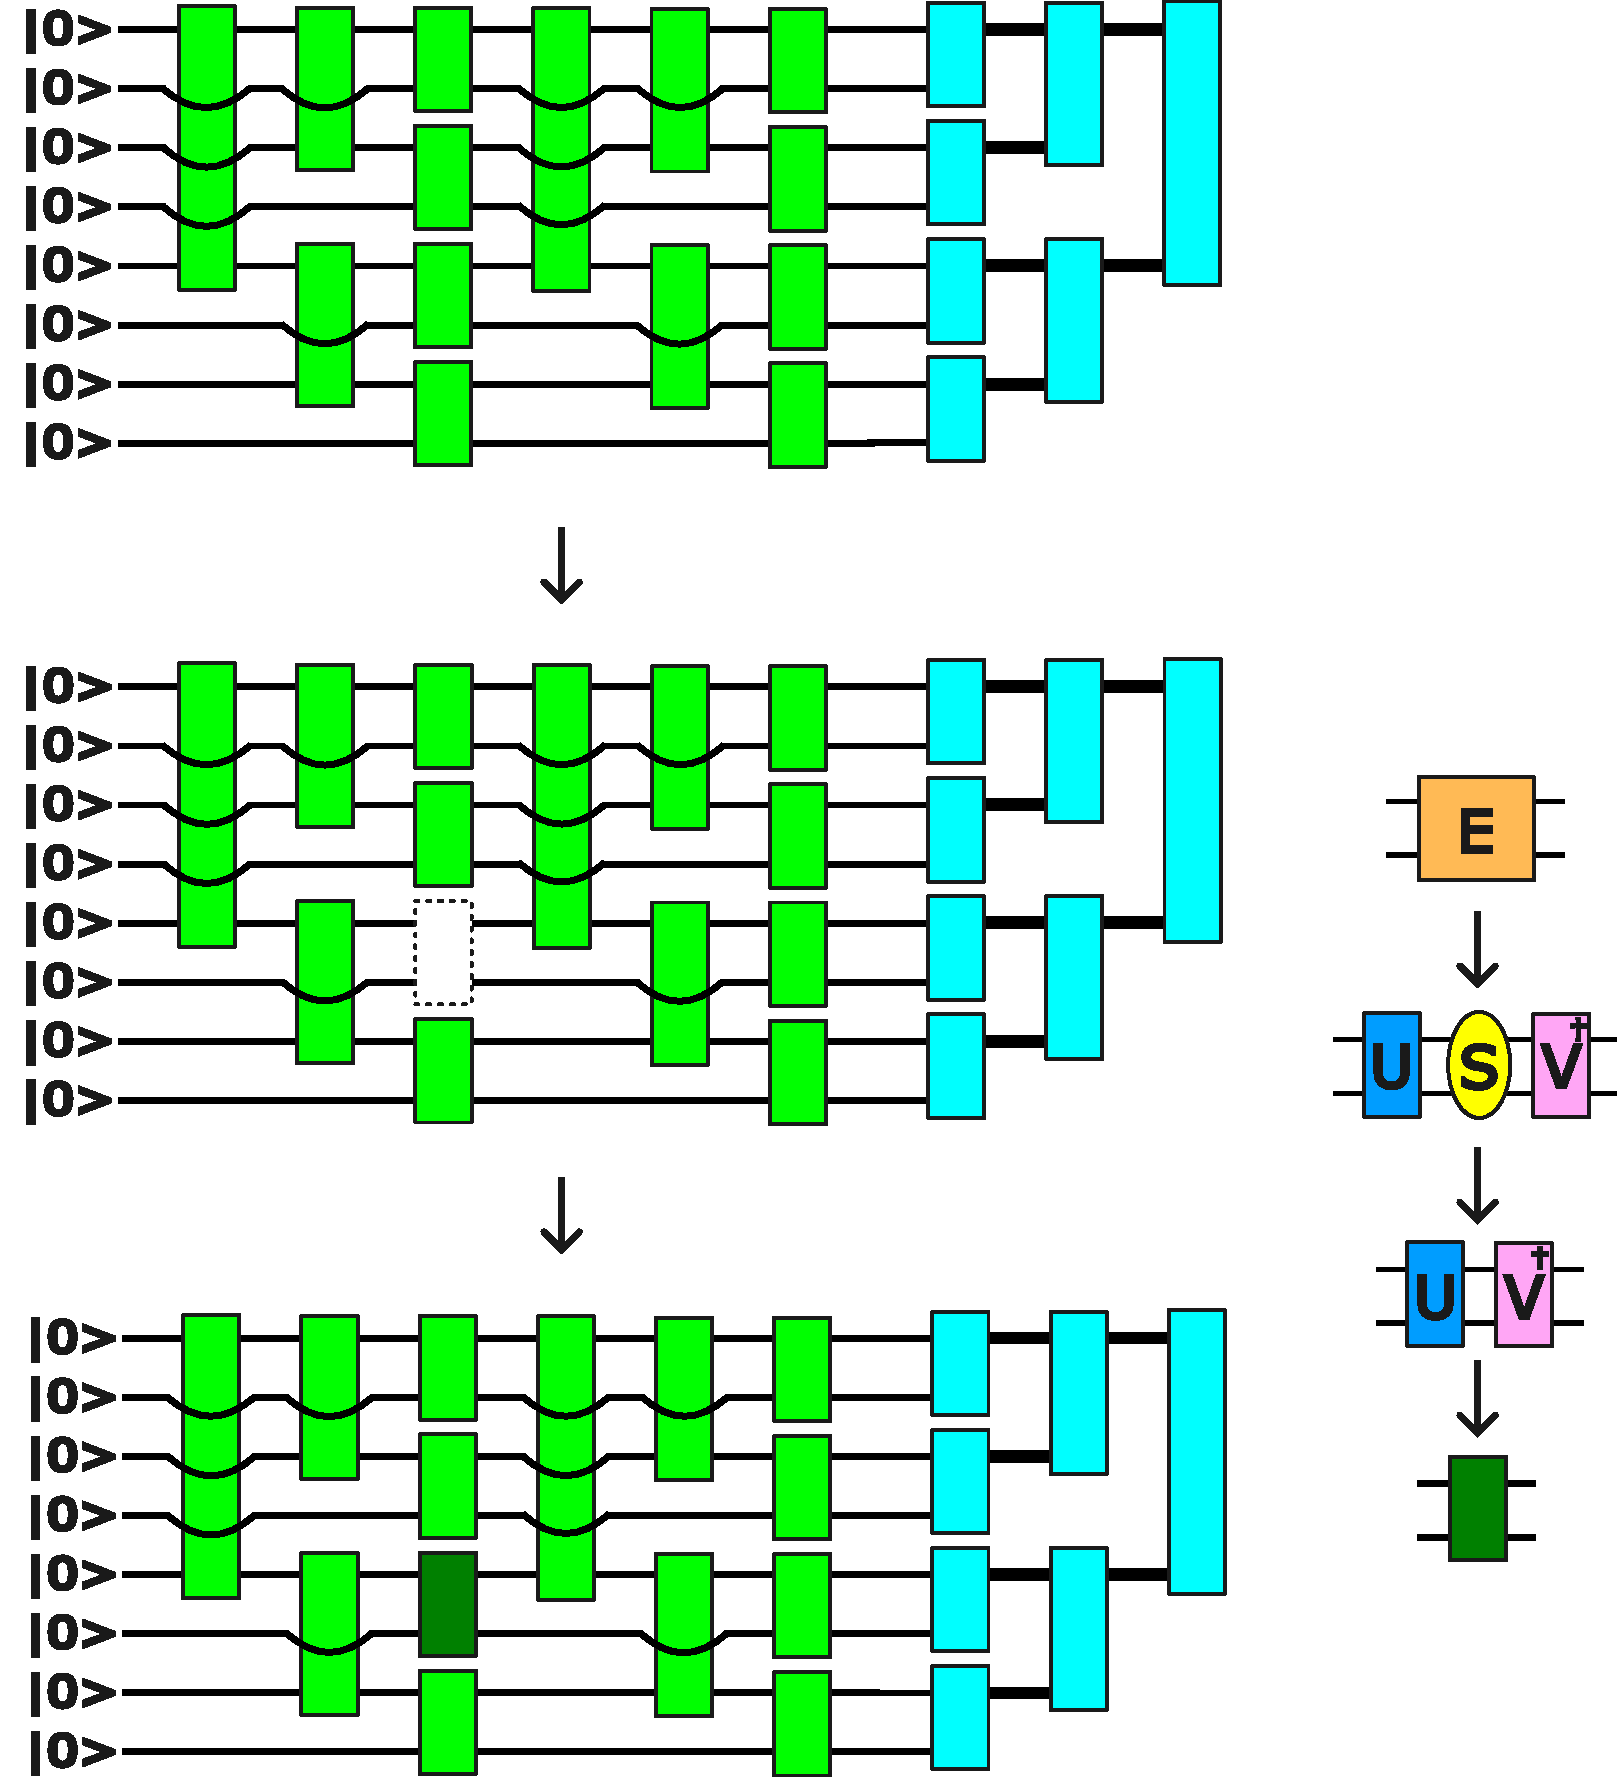
\epsfig{file = fig-optimization.pdf, width = 15cm}}
%   \caption{The environment tensor $E$ is obtained by contracting all tensors except the one of interest. We compute its SVD $E=USV^\dagger$ and calculate $UV^\dagger$ to find the unitary operator closest to the environment tensor. The generated unitary operator is positioned at the location of the removed unitary operator.}
%   \label{fig:optimization}
% \end{figure*}
\begin{figure}
    \centering
    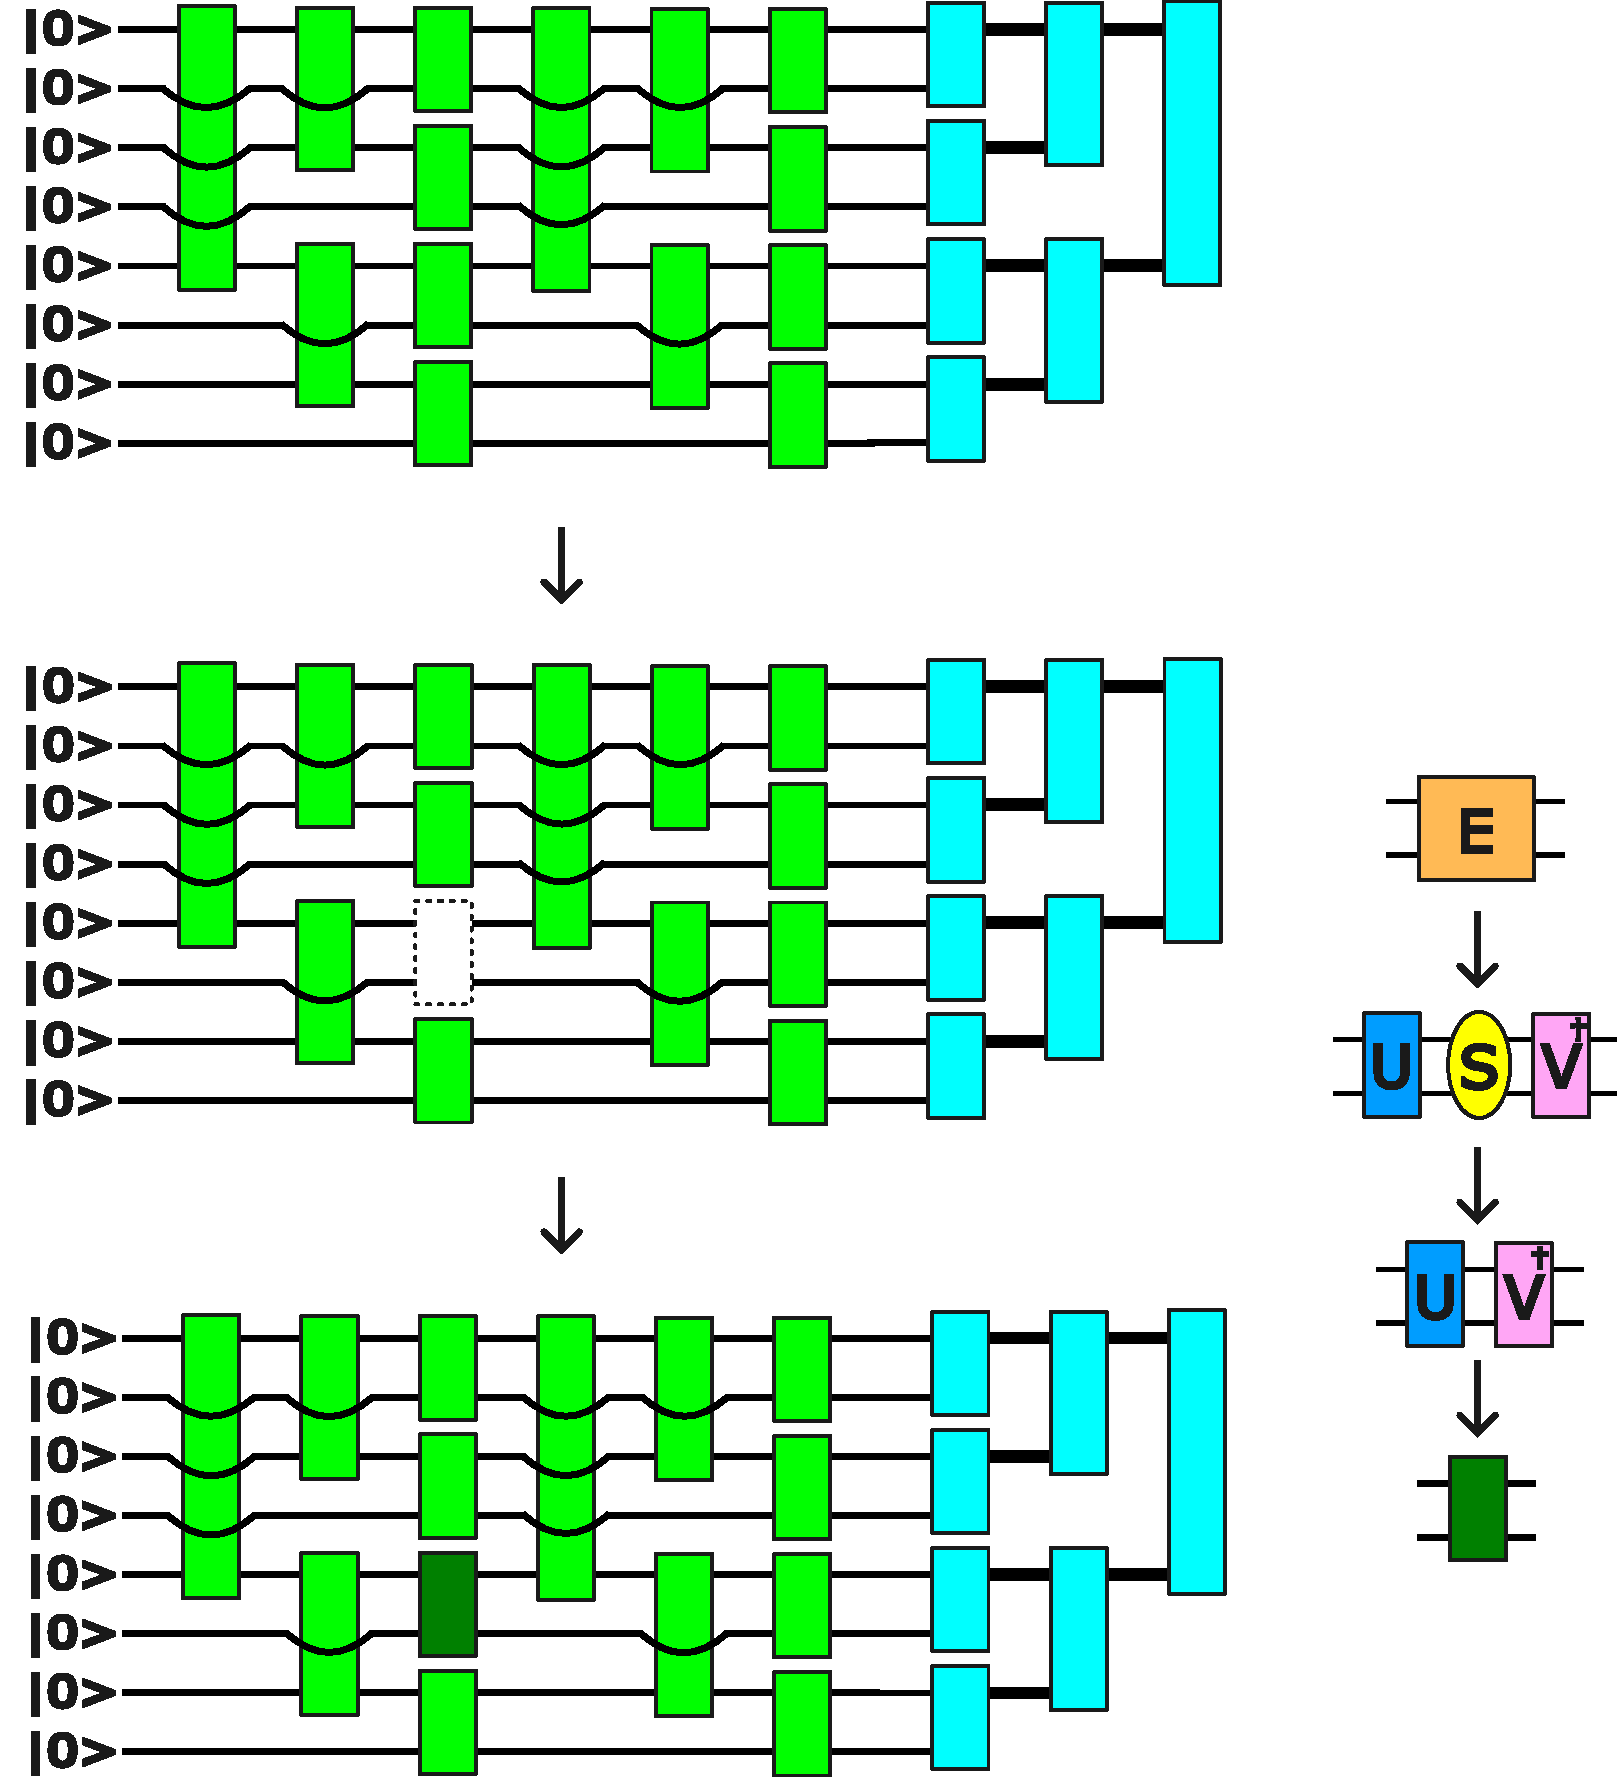
\includegraphics[width=\linewidth]{fig-optimization.pdf}
    \caption{Optimization procedure of tensors. The environment tensor $E$ is obtained by contracting all tensors except the one of interest. We compute its SVD $E=USV^\dagger$ and calculate $UV^\dagger$ to find the unitary operator closest to the environment tensor. The generated unitary operator is positioned at the location of the removed unitary operator.}
    \label{fig:optimization}
\end{figure}
The environment tensor $E$ is obtained by contracting all tensors except for the one of interest.
In this algorithm, the tensor of interest is $\mathrm{L}[U]^{(k)}_i$, and $E$ becomes a four-dimensional tensor with two legs on the left and two on the right.
This tensor represents the optimal operator for maximizing the magnitude of the inner product between the original TTN and the generated quantum circuit.
However, since $E$ is not inherently unitary, it cannot be directly used as a quantum gate.
To address this, we compute SVD of $E$ and utilize the fact that the product $UV^\dagger$ is the unitary matrix that minimizes the Frobenius distance to $E$.
Consequently, $UV^\dagger$ can be considered the unitary operator that maximizes the magnitude of the inner product between the original TTN and the generated quantum circuit.
Given the strength of this local update, we introduce a learning rate $r$, which modifies the unitary update rule via $U_{old}(U_{old}^\dagger U_{new})^r$. 
Replacing $\mathrm{L}[U]^{(k)}_i$ with the unitary operator calculated in this manner for all operators constitutes one step, and repeating this process for $T$ steps completes the optimization algorithm.

The integration of the analytical decomposition and optimization algorithms involves a method where a new layer is added using the analytical decomposition algorithm, followed by optimizing the entire quantum circuit with the optimization algorithm.
This process is repeated iteratively.
\cite{mpsdecomp} refers to this method as Iter[$D_i$, $O_{all}$], confirming that it achieves the highest accuracy regardless of the type of MPSs.
When creating the $(k+1)$-th layer using the analytical decomposition algorithm, the layers up to $k$ are first absorbed into the original TTN using the penetration algorithm before executing the analytical decomposition algorithm.
It should be noted that since we are using the penetration algorithm, the $\ket{\psi}$ that has absorbed $L[U]^{j\dagger}$ retains its TTN structure.
The integrated algorithm is presented as Algorithm~\ref{algorithm:integration}.
\begin{algorithm}[tbp]
 \caption{[$D_i$, $O_{all}$] method for TTN}
 \label{algorithm:integration}
 \KwIn{TTN $\psi_0$, Maximum number of layers $K$}
 \KwOut{Quantum Circuit $\prod_{k=1}^K \mathrm{L}[U]^{(k)}\ket{0}$}
 $\ket{\psi} \leftarrow{\ket{\psi_0}}$\;
 \For{$k=1$ to $K$}{
 Truncate $\ket{\psi}$ to $\ket{\psi_{\chi=2}}$ via SVD\;
 Convert $\ket{\psi_{\chi=2}}$ to $\mathrm{L}[U]^{(k)}$\;
 Optimize $\prod_{k'=1}^{k} \mathrm{L}[U]^{(k')}$\;
 \For{$j=1$ to $k$}{
 Absorb $\mathrm{L}[U]^{j\dagger}$ into $\ket{\psi}$\;
 }
 }
\end{algorithm}

\section{Computational complexity}
For a TTN with a maximum bond dimension $\chi$, the memory requirements scale as $\mathcal{O}(N\chi^3)$.
However, the computational complexity of transforming the TTN into its canonical form scale as $\mathcal{O}(N\chi^4)$.
Most of the algorithms related to TTNs require transformation into the canonical form.
Therefore, it is reasonable to assume that we set $\chi$ such that computations of $\mathcal{O}(N\chi^4)$ can be performed efficiently.

In Algorithm~\ref{algorithm:integration}, truncating $\ket{\psi}$ to $\ket{\psi_{\chi=2}}$ requires $\mathcal{O}(N\chi^3)$.
Optimizing the entire circuit is significantly more challenging compared to MPS due to the complexity of the TTN structure.
Generally, exponential memory is required with respect to $N$, but by using an appropriate contraction order and caching, the computation can be performed in $\mathcal{O}(N\chi^3 4^K)$, which is linear in $N$.
Although the computational complexity increases exponentially with the number of layers, this algorithm is designed for embedding into shallow quantum circuits, and it operates efficiently for $K \approx 7$, as used in our experiments.
Furthermore, when embedding TTNs into a larger number of layers, it is possible to achieve $\mathcal{O}(N\log{N}\chi^4KT)$, where $T$ is the number of sweeps, linear computational complexity with respect to the number of layers, bond dimension by introducing approximations that prevent the bond dimension from exceeding $\chi$ during the contraction of environment tensors, as used in the embedding of MPS~\cite{mpsdecomp}.

The computational complexity of absorbing $K$ layers into the original TTN is $\mathcal{O}(N\log{N}\chi^4K)$.
In the penetration algorithm, SVD of a matrix with row dimension $\chi^2$ and column dimension $\chi$ has a complexity of $\mathcal{O}(\chi^4)$.
Given that the depth of the TTN is $\mathcal{O}(\log{N})$, the penetration operation is performed $\mathcal{O}(\log{N})$ times per tensor.
Since each layer contains $\mathcal{O}(N)$ tensors, the complexity of absorbing one layer is $\mathcal{O}(N\log{N}\chi^4)$, leading to a total complexity of $\mathcal{O}(N\log{N}\chi^4K)$ for $K$ layers.
In summary, the computational complexity to generate one layer is $\mathcal{O}(\max (N\log{N}\chi^4 K, N\chi^3 4^K))$, and it is $\mathcal{O}(\max (N\log{N}\chi^4 K^2, N\chi^3 4^K))$ for $K$ layers.
It scales with the number of qubits.
Additionally, the bond dimension is constrained to $\chi^4$, making it suitable for embedding TTNs with large bond dimensions.
Furthermore, by allowing approximations in optimization, the complexity can be reduced to $\mathcal{O}(N\log{N}\chi^4 K^2T)$ for $K$ layers.
% 基本的な流れはMPSの場合と同様であること

% MPSの場合と異なるのはcontractionが大変であること

% \section{Penetration algorithm}

% \section{Computational complexity}
% MPSの場合の計算量と同じように書く

% \cleardoublepage
% \chapter{Further improvements to the decomposition algorithm with a focus on optimization}
% 既存のdisentanglerではランダムベクトルを作用させていて収束精度に悪影響を与えていること

% decomposeの時点でoptimizationを見据えることで浅いレイヤーで更なる精度向上が期待できること

% optimizationを見据えた手法の説明

\cleardoublepage
\chapter{Numerical Results}
We conducted experiments using two distinct state vectors from the fields of machine learning and physics.
The first state vector represents a uniform superposition over the binary data samples in the $4 \times 4$ bars and stripes (BAS) dataset, which has become a canonical benchmark for generative modeling tasks in quantum machine learning.
The second state vector represents the ground state of the $J_1$-$J_2$ Heisenberg model, a model that characterizes competing interactions in quantum spin systems.
The Hamiltonian for this model is given by
\begin{equation}
    H=J_1 \sum_{<i,j>} \bm{S}_i \cdot \bm{S}_j + J_2 \sum_{<<i,j>>} \bm{S}_i \cdot \bm{S}_j,
\end{equation}
where $J_1(J_2)$ represents the nearest~(next-nearest) neighbor interactions. 
By varying the ratio of the first and second nearest-neighbor interactions, the $J_1$-$J_2$ Heisenberg model exhibits complex quantum many-body phenomena and has been widely studied.
In this thesis, we utilized $J_2/J_1=0.5$.
Both state vectors have two-dimensional correlations, making them more suitably represented by TTNs rather than MPSs.

The state vector of the BAS was manually prepared, while the ground state of the $J_1$-$J_2$ Heisenberg model was generated using a numerical solver package $\mathcal{H}\Phi$~\cite{hphi}, which is designed for a wide range of quantum lattice models. 
MPSs and TTNs were constructed by iteratively applying SVD to the state vector from the edges.
% The maximum bond dimension $\chi$ was set to eight.

The conversion from MPSs and TTNs to quantum circuits employed the Iter[$D_i$, $O_{all}$] method, which is also utilized in the proposed method.
Additionally, to compare with the proposed method, we also used $D_{all}$, $O_{all}$, and Iter[$I_i$, $O_{all}$] from \cite{mpsdecomp}.
The $D_{all}$ method generates circuits solely through analytical decomposition.
The $O_{all}$ method optimizes circuits starting from an initial state composed only of identity gates.
The Iter[$I_i$, $O_{all}$] method sequentially adds identity layers, optimizing the entire circuit at each step.
% We set the hyperparameters to 1,000 optimization sweeps and a learning rate of 0.6.

To measure the accuracy of embedding into quantum circuits, we utilized infidelity as the evaluation metric.
The infidelity $I_f$ between two quantum states, $\ket{\Psi}$ and $\ket{\Phi}$, is expressed as
\begin{equation}
    I_f = 1 - |\braket{\Phi|\Psi}|,
\end{equation}
and a smaller infidelity indicates that the two quantum states are closer.
In this study, infidelity quantifies the success of our transformations.
% \begin{figure}[!h]
%   \centering
%    {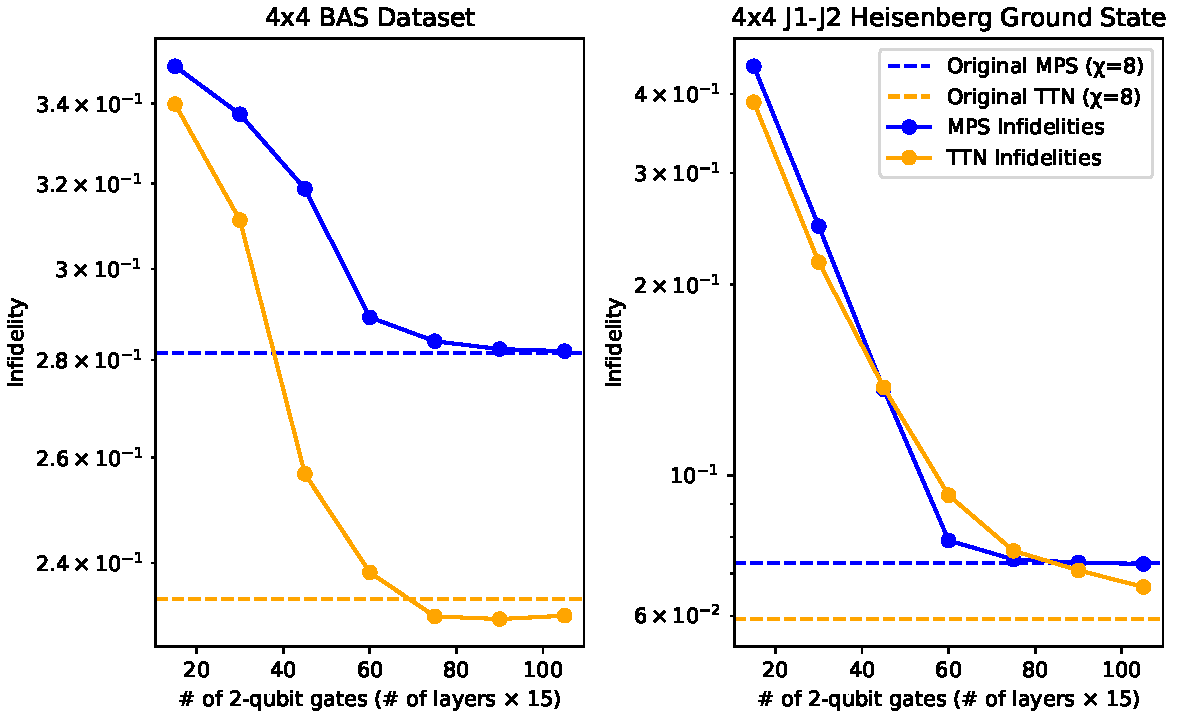
\epsfig{file = fig_ttn_mps.pdf, width = 7cm}}
%   \caption{Infidelities between original state vectors and generated quantum circuits. The bond dimensions of tensor networks are eight and the number of optimization steps is 1,000. The learning rate for optimization is set to 0.65 for the BAS Dataset and 0.6 for the $J_1$-$J_2$ Heisenberg model. MPS is represented by the blue line, while TTN is depicted by the orange line. Additionally, the infidelity between the tensor network and the state vector is indicated by the dotted line.}
%   \label{fig:result1}
%  \end{figure}
 \begin{figure}
    \centering
    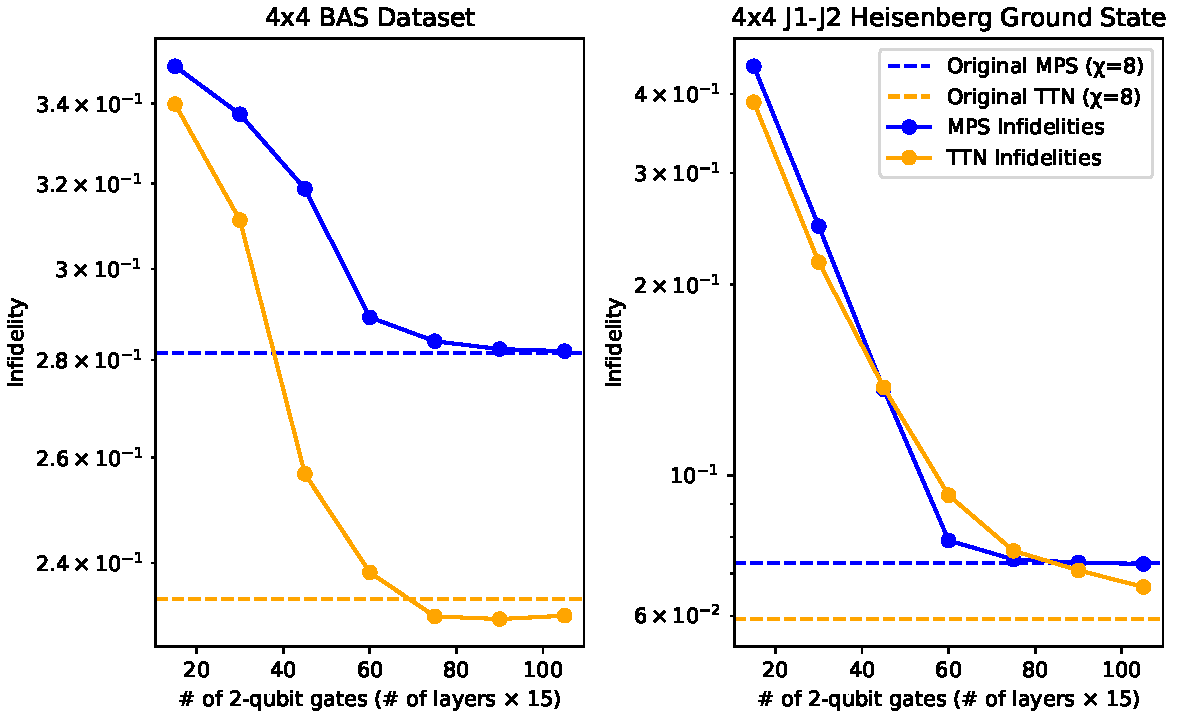
\includegraphics[width=\linewidth]{fig_ttn_mps.pdf}
    \caption{Infidelities between original state vectors and generated quantum circuits. The bond dimensions of tensor networks are 8, and the number of optimization steps is 1,000. The learning rate for optimization is set to 0.65 for the BAS dataset and 0.6 for the $J_1$-$J_2$ Heisenberg model. The MPS results are represented by the blue lines, while the TTN results are depicted by the orange lines. Additionally, the infidelity between the tensor network and the state vector is indicated by the dotted lines.}
    \label{fig:result1}
\end{figure}
 
 % \begin{figure}[!h]
 %  \centering
 %   {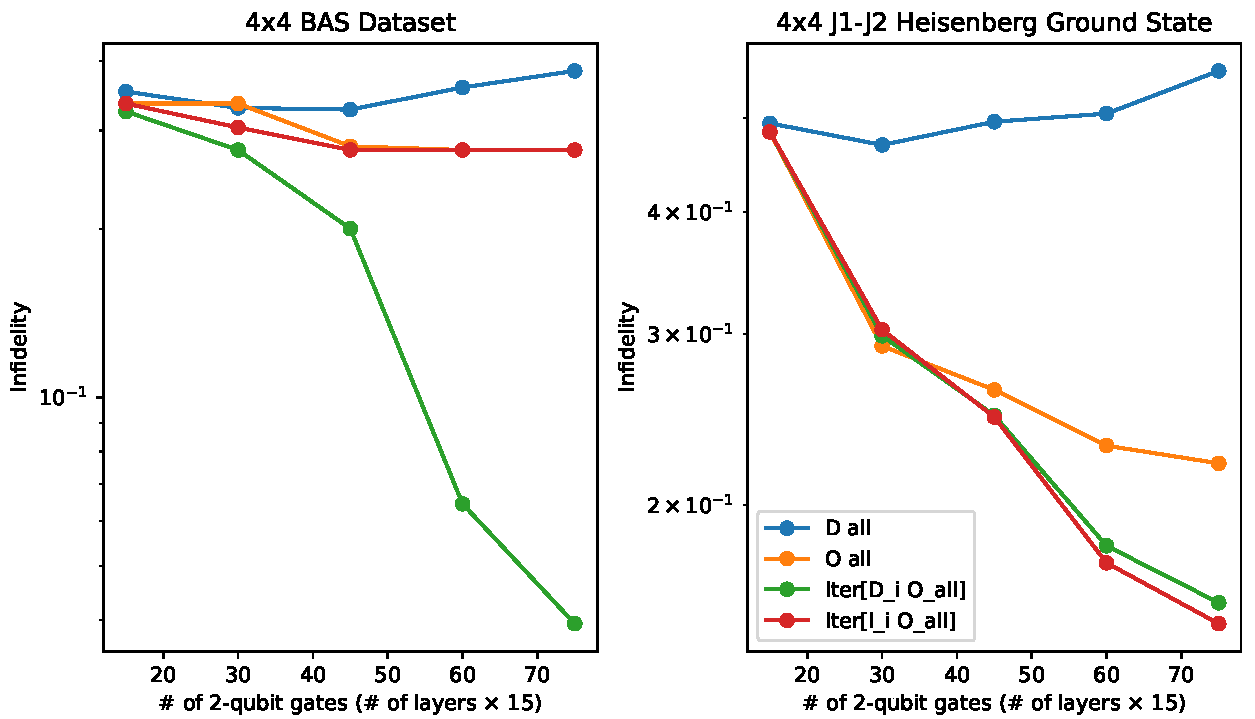
\epsfig{file = fig_optim_type, width = 7cm}}
 %  \caption{Infidelities between original TTNs and generated quantum circuits. The bond dimensions of TTNs are 16 and the number of optimization steps is 1,000. The learning rate for optimization is set to 0.6.}
 %  \label{fig:result2}
 % \end{figure}
  \begin{figure}
    \centering
    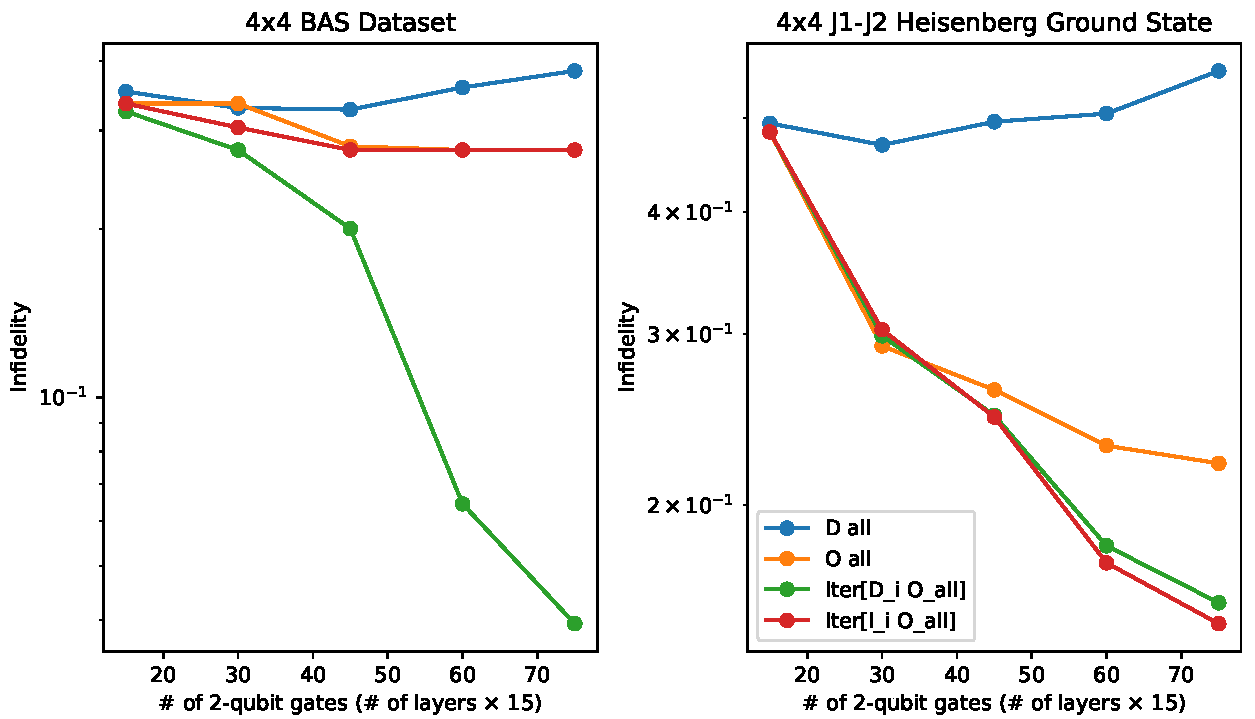
\includegraphics[width=\linewidth]{fig_optim_type.pdf}
    \caption{Infidelities between original TTNs and generated quantum circuits. The bond dimensions of TTNs are 16, and the number of optimization steps is 1,000. The learning rate for optimization is set to 0.6.}
    \label{fig:result2}
\end{figure}


Figure~\ref{fig:result1} illustrates the infidelity between the original state vector and the quantum circuits embedded with either TTN or MPS.
Despite the greater difficulty in embedding TTNs into shallow quantum circuits due to their hierarchical structure, the infidelities between original state vectors and generated quantum circuits from TTNs are sufficiently low, indicating the successful embedding of the TTNs into shallow quantum circuits.
Notably, in the BAS dataset, the TTN's superior representational capacity enables more accurate embeddings than MPS.
% 特に浅い回路やMPSを超える深い回路で性能が高いことに言及

The result of the $J_1$-$J_2$ Heisenberg model reveals an intriguing pattern: TTN outperforms in both shallow and deep quantum circuits, while MPS excels in the intermediate region.
In deep quantum circuits, the superior representational capacity of TTN results in enhanced convergence accuracy.
For shallow and intermediate quantum circuits, this result can be interpreted as a trade-off between representational capacity and approximation error.
Generally, TTN surpasses MPS in representational capacity, enabling the depiction of states that are inadequate for MPS.
However, embedding TTN introduces larger approximation errors than MPS. 
Consequently, in the shallow region, TTN prepares a better initial circuit due to its representational advantage outweighing the approximation error.
Conversely, in the intermediate region, MPS prepares a better initial circuit as the approximation error outweighs the representational capacity. 
As the number of qubits in quantum computers increases, the difference in representational capacity between TTN and MPS will become more pronounced, and the impact of approximation errors will relatively diminish.

Figure~\ref{fig:result2} highlights the importance of the analytical decomposition algorithm for embedding TTNs into quantum circuits.
As demonstrated in previous research on MPS~\cite{mpsdecomp}, methods such as Iter[$D_i$, $O_{all}$] and Iter[$I_i$, $O_{all}$], which sequentially add layers and optimize all circuits, achieve high accuracy. 
Furthermore, as suggested in previous studies, it was confirmed that Iter[$I_i$, $O_{all}$] struggles with the BAS dataset even in TTN embeddings, where the singular values at the bond become discontinuous. 
This indicates that Iter[$D_i$, $O_{all}$] is the most effective and robust embedding method, achieving high accuracy in multiple fields, including machine learning and physics, thus affirming the critical importance of the analytical decomposition algorithm.
This result also verifies the effective performance of the proposed analytical decomposition method.
% 実験で使用したMPS, TTNの作り方

% Iter[D_i, O_all]が最も良いことを示してDecompを考える意義を示す図

% MPSと比較する図

% Optimizationを見据えたdecompの改良で精度が上がることの確認

% 計算時間の結果

\cleardoublepage
\chapter{Conclusion}
To avoid the barren plateau issue in VQAs, there is increasing interest in using tensor networks to initialize quantum circuits. 
However, embedding tensor networks into shallow quantum circuits is generally difficult, and prior research has been limited to embedding MPSs.
In this study, we proposed a method for embedding TTNs, which have a more complex structure than MPSs and can efficiently represent two-dimensional systems and systems with long-range correlations into shallow quantum circuits composed solely of two-qubit gates.
We applied our proposed method to different types of TTNs and confirmed that it prepares quantum circuit parameters with better accuracy than embedding MPSs.
Additionally, the computational complexity is $\mathcal{O}(\max (N\log{N}\chi^4 K^2, N\chi^3 4^K))$, or $\mathcal{O}(N\log{N}\chi^4 K^2T)$ with approximation, making it applicable to practical problems.
This study will be an important bridge for implementing hybrid algorithms combining tree tensor networks and quantum computing.

\bibliographystyle{apalike}
\bibliography{main}


\end{document}